% !TeX spellcheck = pl_PL
%%%%%%%%%%%%%%%%%%%%%%%%%%%%%%%%%%%%%%%%%%%
%                                        %
% Szablon pracy dyplomowej inzynierskiej %
% zgodny  z aktualnymi  przepisami  SZJK %
%                                        %
%%%%%%%%%%%%%%%%%%%%%%%%%%%%%%%%%%%%%%%%%%
%                                        %
%  (c) Krzysztof Simiński, 2018-2023     %
%                                        %
%%%%%%%%%%%%%%%%%%%%%%%%%%%%%%%%%%%%%%%%%%
%                                        %
% Najnowsza wersja szablonów jest        %
% podstępna pod adresem                  %
% github.com/ksiminski/polsl-aei-theses  %
%                                        %
%%%%%%%%%%%%%%%%%%%%%%%%%%%%%%%%%%%%%%%%%%
%
%
% Projekt LaTeXowy zapewnia odpowiednie formatowanie pracy,
% zgodnie z wymaganiami Systemu zapewniania jakości kształcenia.
% Proszę nie zmieniać ustawień formatowania (np. fontu,
% marginesów, wytłuszczeń, kursywy itd. ).
%
% Projekt można kompilować na kilka sposobów.
%
% 1. kompilacja pdfLaTeX
%
% pdflatex main
% bibtex   main
% pdflatex main
% pdflatex main
%
%
% 2. kompilacja XeLaTeX
%
% Kompilatacja przy użyciu XeLaTeXa różni się tym, że na stronie
% tytułowej używany jest font Calibri. Wymaga to jego uprzedniego
% zainstalowania.
%
% xelatex main
% bibtex  main
% xelatex main
% xelatex main
%
%
%%%%%%%%%%%%%%%%%%%%%%%%%%%%%%%%%%%%%%%%%%%%%%%%%%%%%
% W przypadku pytań, uwag, proszę pisać na adres:   %
%      krzysztof.siminski(małpa)polsl.pl            %
%%%%%%%%%%%%%%%%%%%%%%%%%%%%%%%%%%%%%%%%%%%%%%%%%%%%%
%
% Chcemy ulepszać szablony LaTeXowe prac dyplomowych.
% Wypełniając ankietę spod poniższego adresu pomogą
% Państwo nam to zrobić. Ankieta jest całkowicie
% anonimowa. Dziękujemy!


% https://docs.google.com/forms/d/e/1FAIpQLScyllVxNKzKFHfILDfdbwC-jvT8YL0RSTFs-s27UGw9CKn-fQ/viewform?usp=sf_link
%
%%%%%%%%%%%%%%%%%%%%%%%%%%%%%%%%%%%%%%%%%%%%%%%%%%%%%%%%%%%%%%%%%%%%%%%%%

%%%%%%%%%%%%%%%%%%%%%%%%%%%%%%%%%%%%%%%%%%%%%%%
%                                             %
% PERSONALIZACJA PRACY – DANE PRACY           %
%                                             %
%%%%%%%%%%%%%%%%%%%%%%%%%%%%%%%%%%%%%%%%%%%%%%%

% Proszę wpisać swoje dane w poniższych definicjach.

% TODO
% dane autora
\newcommand{\FirstNameAuthor}{Jakub}
\newcommand{\SurnameAuthor}{Pająk}
\newcommand{\IdAuthor}{300566}   % numer albumu  (bez $\langle$ i $\rangle$)

% drugi autor:
%\newcommand{\FirstNameCoauthor}{Imię}   % Jeżeli jest drugi autor, to tutaj należy podać imię.
%\newcommand{\SurnameCoauthor}{Nazwisko} % Jeżeli jest drugi autor, to tutaj należy podać nazwisko.
%\newcommand{\IdCoauthor}{$\langle$wpisać właściwy$\rangle$}  % numer albumu drugiego autora (bez $\langle$ i $\rangle$)
% Gdy nie ma drugiego autora, należy zostawić poniższe definicje puste, jak poniżej. Gdy jest drugi autor, należy zakomentować te linie.
\newcommand{\FirstNameCoauthor}{} % Jeżeli praca ma tylko jednego autora, to dane drugiego autora zostają puste.
\newcommand{\SurnameCoauthor}{}   % Jeżeli praca ma tylko jednego autora, to dane drugiego autora zostają puste.
\newcommand{\IdCoauthor}{}  % Jeżeli praca ma tylko jednego autora, to dane drugiego autora zostają puste.
%%%%%%%%%%

\newcommand{\Supervisor}{dr inż. Krzysztof Jaskot}     % dane promotora (bez $\langle$ i $\rangle$)
\newcommand{\Title}{Zrobotyzowany system sortowania klocków}           % tytuł pracy po polsku
\newcommand{\TitleAlt}{Robotic brick sorting system}                     % thesis title in English
\newcommand{\Program}{Automatyka i Robotyka}            % kierunek studiów  (bez $\langle$ i $\rangle$)
\newcommand{\Specialisation}{Technologie Informacyjne w Automatyce i Robotyce}     % specjalność  (bez $\langle$ i $\rangle$)
\newcommand{\Departament}{Automatyki i Robotyki}        % katedra promotora  (bez $\langle$ i $\rangle$)

% Jeżeli został wyznaczony promotor pomocniczy lub opiekun, proszę go/ją wpisać ...
%\newcommand{\Consultant}{$\langle$stopień naukowy imię i nazwisko$\rangle$} % dane promotora pomocniczego, opiekuna (bez $\langle$ i $\rangle$)
% ... w przeciwnym razie proszę zostawić puste miejsce jak poniżej:
\newcommand{\Consultant}{} % brak promotowa pomocniczego / opiekuna

% koniec fragmentu do modyfikacji
%%%%%%%%%%%%%%%%%%%%%%%%%%%%%%%%%%%%%%%%%%


%%%%%%%%%%%%%%%%%%%%%%%%%%%%%%%%%%%%%%%%%%%%%%%
%                                             %
% KONIEC PERSONALIZACJI PRACY                 %
%                                             %
%%%%%%%%%%%%%%%%%%%%%%%%%%%%%%%%%%%%%%%%%%%%%%%

%%%%%%%%%%%%%%%%%%%%%%%%%%%%%%%%%%%%%%%%


%%%%%%%%%%%%%%%%%%%%%%%%%%%%%%%%%%%%%%%%%%%%%%%
%                                             %
% PROSZĘ NIE MODYFIKOWAĆ PONIŻSZYCH USTAWIEŃ! %
%                                             %
%%%%%%%%%%%%%%%%%%%%%%%%%%%%%%%%%%%%%%%%%%%%%%%



\documentclass[a4paper,twoside,12pt]{book}
\usepackage[utf8]{inputenc}                                      
\usepackage[T1]{fontenc}  
\usepackage{amsmath,amsfonts,amssymb,amsthm}
\usepackage[british,polish]{babel} 
\usepackage{indentfirst}
\usepackage{xurl}
\usepackage{xstring}
\usepackage{ifthen}



\usepackage{ifxetex}

\ifxetex
	\usepackage{fontspec}
	\defaultfontfeatures{Mapping=tex—text} % to support TeX conventions like ``——-''
	\usepackage{xunicode} % Unicode support for LaTeX character names (accents, European chars, etc)
	\usepackage{xltxtra} % Extra customizations for XeLaTeX
\else
	\usepackage{lmodern}
\fi



\usepackage[margin=2.5cm]{geometry}
\usepackage{graphicx} 
\usepackage{hyperref}
\usepackage{booktabs}
\usepackage{tikz}
\usepackage{pgfplots}
\usepackage{mathtools}
\usepackage{geometry}
\usepackage{subcaption}   % subfigures
\usepackage[page]{appendix} % toc,
\renewcommand{\appendixtocname}{Dodatki}
\renewcommand{\appendixpagename}{Dodatki}
\renewcommand{\appendixname}{Dodatek}

\usepackage{csquotes}
\usepackage[natbib=true,backend=bibtex,maxbibnames=99]{biblatex}  % kompilacja bibliografii BibTeXem
%\usepackage[natbib=true,backend=biber,maxbibnames=99]{biblatex}  % kompilacja bibliografii Biberem
\bibliography{biblio/biblio}

\usepackage{ifmtarg}   % empty commands  

\usepackage{setspace}
\onehalfspacing


\frenchspacing



%%%% TODO LIST GENERATOR %%%%%%%%%

\usepackage{color}
\definecolor{brickred}      {cmyk}{0   , 0.89, 0.94, 0.28}

\makeatletter \newcommand \kslistofremarks{\section*{Uwagi} \@starttoc{rks}}
  \newcommand\l@uwagas[2]
    {\par\noindent \textbf{#2:} %\parbox{10cm}
{#1}\par} \makeatother


\newcommand{\ksremark}[1]{%
{%\marginpar{\textdbend}
{\color{brickred}{[#1]}}}%
\addcontentsline{rks}{uwagas}{\protect{#1}}%
}

\newcommand{\comma}{\ksremark{przecinek}}
\newcommand{\nocomma}{\ksremark{bez przecinka}}
\newcommand{\styl}{\ksremark{styl}}
\newcommand{\ortografia}{\ksremark{ortografia}}
\newcommand{\fleksja}{\ksremark{fleksja}}
\newcommand{\pauza}{\ksremark{pauza `--', nie dywiz `-'}}
\newcommand{\kolokwializm}{\ksremark{kolokwializm}}
\newcommand{\cudzyslowy}{\ksremark{,,polskie cudzysłowy''}}

%%%%%%%%%%%%%% END OF TODO LIST GENERATOR %%%%%%%%%%%

\newcommand{\printCoauthor}{%		
    \StrLen{\FirstNameCoauthor}[\FNCoALen]
    \ifthenelse{\FNCoALen > 0}%
    {%
		{\large\bfseries\Coauthor\par}
	
		{\normalsize\bfseries \LeftId: \IdCoauthor\par}
    }%
    {}
} 

%%%%%%%%%%%%%%%%%%%%%
\newcommand{\autor}{%		
    \StrLen{\FirstNameCoauthor}[\FNCoALenXX]
    \ifthenelse{\FNCoALenXX > 0}%
    {\FirstNameAuthor\ \SurnameAuthor, \FirstNameCoauthor\ \SurnameCoauthor}%
	{\FirstNameAuthor\ \SurnameAuthor}%
}
%%%%%%%%%%%%%%%%%%%%%

\StrLen{\FirstNameCoauthor}[\FNCoALen]
\ifthenelse{\FNCoALen > 0}%
{%
\author{\FirstNameAuthor\ \SurnameAuthor, \FirstNameCoauthor\ \SurnameCoauthor}
}%
{%
\author{\FirstNameAuthor\ \SurnameAuthor}
}%

%%%%%%%%%%%% ZYWA PAGINA %%%%%%%%%%%%%%%
% brak kapitalizacji zywej paginy
\usepackage{fancyhdr}
\pagestyle{fancy}
\fancyhf{}
\fancyhead[LO]{\nouppercase{\it\rightmark}}
\fancyhead[RE]{\nouppercase{\it\leftmark}}
\fancyhead[LE,RO]{\it\thepage}


\fancypagestyle{tylkoNumeryStron}{%
   \fancyhf{} 
   \fancyhead[LE,RO]{\it\thepage}
}

\fancypagestyle{bezNumeracji}{%
   \fancyhf{} 
   \fancyhead[LE,RO]{}
}


\fancypagestyle{NumeryStronNazwyRozdzialow}{%
   \fancyhf{} 
   \fancyhead[LE]{\nouppercase{\autor}}
   \fancyhead[RO]{\nouppercase{\leftmark}} 
   \fancyfoot[CE, CO]{\thepage}
}


%%%%%%%%%%%%% OBCE WTRETY  
\newcommand{\obcy}[1]{\emph{#1}}
\newcommand{\english}[1]{{\selectlanguage{british}\obcy{#1}}}
%%%%%%%%%%%%%%%%%%%%%%%%%%%%%

% polskie oznaczenia funkcji matematycznych
\renewcommand{\tan}{\operatorname {tg}}
\renewcommand{\log}{\operatorname {lg}}

% jeszcze jakies drobiazgi

\newcounter{stronyPozaNumeracja}

%%%%%%%%%%%%%%%%%%%%%%%%%%% 
\newcommand{\printOpiekun}[1]{%		

    \StrLen{\Consultant}[\mystringlen]
    \ifthenelse{\mystringlen > 0}%
    {%
       {\large{\bfseries OPIEKUN, PROMOTOR POMOCNICZY}\par}
       
       {\large{\bfseries \Consultant}\par}
    }%
    {}
} 
%
%%%%%%%%%%%%%%%%%%%%%%%%%%%%%%%%%%%%%%%%%%%%%%
 
% Proszę nie modyfikować poniższych definicji!
\newcommand{\Author}{\FirstNameAuthor\ \MakeUppercase{\SurnameAuthor}} 
\newcommand{\Coauthor}{\FirstNameCoauthor\ \MakeUppercase{\SurnameCoauthor}}
\newcommand{\Type}{PROJEKT INŻYNIERSKI}
\newcommand{\Faculty}{Wydział Automatyki, Elektroniki i Informatyki} 
\newcommand{\Polsl}{Politechnika Śląska}
\newcommand{\Logo}{graf/politechnika_sl_logo_bw_pion_pl.pdf}
\newcommand{\LeftId}{Nr albumu}
\newcommand{\LeftProgram}{Kierunek}
\newcommand{\LeftSpecialisation}{Specjalność}
\newcommand{\LeftSUPERVISOR}{PROWADZĄCY PRACĘ}
\newcommand{\LeftDEPARTMENT}{KATEDRA}
%%%%%%%%%%%%%%%%%%%%%%%%%%%%%%%%%%%%%%%%%%%%%%

%%%%%%%%%%%%%%%%%%%%%%%%%%%%%%%%%%%%%%%%%%%%%%%
%                                             %
% KONIEC USTAWIEŃ                             %
%                                             %
%%%%%%%%%%%%%%%%%%%%%%%%%%%%%%%%%%%%%%%%%%%%%%%

 % Proszę nie modyfikować pliku settings.tex


%%%%%%%%%%%%%%%%%%%%%%%%%%%%%%%%%%%%%%%%%%%%%%%
%                                             %
% MOJE PAKIETY, USTAWIENIA ITD                %
%                                             %
%%%%%%%%%%%%%%%%%%%%%%%%%%%%%%%%%%%%%%%%%%%%%%%

% Tutaj proszę umieszczać swoje pakiety, makra, ustawienia itd.


 
%%%%%%%%%%%%%%%%%%%%%%%%%%%%%%%%%%%%%%%%%%%%%%%%%%%%%%%%%%%%%%%%%%%%%
% listingi i fragmentu kodu źródłowego 
% pakiet: listings lub minted
% % % % % % % % % % % % % % % % % % % % % % % % % % % % % % % % % % % 

% biblioteka listings
\usepackage{listings}
\lstset{%
morekeywords={string,exception,std,vector},% słowa kluczowe rozpoznawane przez pakiet listings
language=C++, Python, bash % C, Matlab, Python, SQL, TeX, XML, bash, ... – vide https://www.ctan.org/pkg/listings
commentstyle=\textit,%
identifierstyle=\textsf,%
keywordstyle=\sffamily\bfseries, %\texttt, %
%captionpos=b,%
tabsize=3,%
frame=lines,%
numbers=left,%
numberstyle=\tiny,%
numbersep=5pt,%
breaklines=true,%
escapeinside={@*}{*@},%
}

\usepackage{float}

\tolerance=1 
\emergencystretch=\maxdimen 
\hyphenpenalty=10000 
\hbadness=10000

\renewcommand{\lstlistingname}{Fragment kodu}


% \usepackage[draft,nosingleletter]{impnattypo}
% \babelprovide[transforms = oneletter.nobreak]{polish} 

% % % % % % % % % % % % % % % % % % % % % % % % % % % % % % % % % % % 
% pakiet minted
%\usepackage{minted}

% pakiet wymaga specjalnego kompilowania:
% pdflatex -shell-escape main.tex
% xelatex  -shell-escape main.tex

%\usepackage[chapter]{minted} % [section]
%%\usemintedstyle{bw}   % czarno-białe kody 
%
%\setminted % https://ctan.org/pkg/minted
%{
%%fontsize=\normalsize,%\footnotesize,
%%captionpos=b,%
%tabsize=3,%
%frame=lines,%
%framesep=2mm,
%numbers=left,%
%numbersep=5pt,%
%breaklines=true,%
%escapeinside=@@,%
%}

%%%%%%%%%%%%%%%%%%%%%%%%%%%%%%%%%%%%%%%%%%%%%%%%%%%%%%%%%%%%%%%%%%%%%



%%%%%%%%%%%%%%%%%%%%%%%%%%%%%%%%%%%%%%%%%%%%%%%
%                                             %
% KONIEC MOICH USTAWIEŃ                       %
%                                             %
%%%%%%%%%%%%%%%%%%%%%%%%%%%%%%%%%%%%%%%%%%%%%%%

 % Tutaj proszę umieścić swoje pakiety, makra, ustawienia itd.

%%%%%%%%%%%%%%%%%%%%%%%%%%%%%%%%%%%%%%%%


\begin{document}
%\kslistofremarks

\frontmatter

%%%%%%%%%%%%%%%%%%%%%%%%%%%%%%%%%%%%%%%%%%%%%%%
%                                             %
% PROSZĘ NIE MODYFIKOWAĆ STRONY TYTUŁOWEJ!    %
%                                             %
%%%%%%%%%%%%%%%%%%%%%%%%%%%%%%%%%%%%%%%%%%%%%%%


%%%%%%%%%%%%%%%%%%  STRONA TYTUŁOWA %%%%%%%%%%%%%%%%%%%
\pagestyle{empty}
{
	\newgeometry{top=1.5cm,%
	             bottom=2.5cm,%
	             left=3cm,
	             right=2.5cm}
 
	\ifxetex 
	  \begingroup
	  \setsansfont{Calibri}
	   
	\fi 
	 \sffamily
	\begin{center}
	\includegraphics[width=50mm]{\Logo}
	 
	
	{\Large\bfseries\Type\par}
	
	\vfill  \vfill  
			 
	{\large\Title\par}
	
	\vfill  
		
	{\large\bfseries\Author\par}
	
	{\normalsize\bfseries \LeftId: \IdAuthor}

	\printCoauthor
	
	\vfill  		
 
	{\large{\bfseries \LeftProgram:} \Program\par} 
	
	{\large{\bfseries \LeftSpecialisation:} \Specialisation\par} 
	 		
	\vfill  \vfill 	\vfill 	\vfill 	\vfill 	\vfill 	\vfill  
	 
	{\large{\bfseries \LeftSUPERVISOR}\par}
	
	{\large{\bfseries \Supervisor}\par}
				
	{\large{\bfseries \LeftDEPARTMENT\ \Departament} \par}
		
	{\large{\bfseries \Faculty}\par}
		
	\vfill  \vfill  

    	
    \printOpiekun{\Consultant}
    
	\vfill  \vfill  
		
    {\large\bfseries  Gliwice \the\year}

   \end{center}	
       \ifxetex 
       	  \endgroup
       \fi
	\restoregeometry
}
  
%%%%%%%%%%%%%%%%%%%%%%%%%%%%%%%%%%%%%%%%%%%%%%%
%                                             %
% KONIEC STRONY TYTUŁOWEJ                     %
%                                             %
%%%%%%%%%%%%%%%%%%%%%%%%%%%%%%%%%%%%%%%%%%%%%%%  
  % Proszę nie modyfikować pliku titlepage.tex

\cleardoublepage

\rmfamily\normalfont
\pagestyle{empty}


%%% No to zaczynamy pisać pracę :-) %%%%

% TODO
\subsubsection*{Tytuł pracy} 
\Title

\subsubsection*{Streszczenie}  
Celem projektu jest wykonanie autonomicznej platformy jezdnej, mającej na celu
bezobsługowe sortowanie klocków spadających w określone miejsce z taśmociągu lub
innego podajnika. Robot korzystając z możliwości wizji komputerowej będzie
rozpoznawać kolor aktualnego klocka, a następnie na podstawie określonego koloru
będzie wybierać trasę do odpowiedniego pojemnika. Domyślnie rozpoznawane będą trzy
kolory (czerwony, zielony, niebieski) oraz trzy pojemniki, odpowiednie dla każdego koloru.
Wymagania: znajomość programowania układów SBC (Raspberry Pi), Python, OpenCV


\subsubsection*{Słowa kluczowe} 
Robot mobilny, analiza wizyjna, Programowanie mikrokontrolerów

\subsubsection*{Thesis title} 
\begin{otherlanguage}{british}
\TitleAlt
\end{otherlanguage}

\subsubsection*{Abstract} 
\begin{otherlanguage}{british}
    The goal of this project is to create an autonomous mobile platform designed for
    unattended sorting of blocks falling into a designated area from a conveyor belt or
    another feeder. The robot will use computer vision to recognize the color of the
    current block and, based on the identified color, will choose the path to the
    appropriate container. By default, three colors (red, green, blue) will be recognized,
    and there will be three containers, each corresponding to one of the colors.
    Requirements: knowledge of SBC programming (Raspberry Pi), Python, OpenCV
\end{otherlanguage}
\subsubsection*{Key words}  
\begin{otherlanguage}{british}
Mobile robot, visual analysis, microcontroller programming
\end{otherlanguage}

 % informacje redakcyjne


%%%%%%%%%%%%%%%%%% SPIS TRESCI %%%%%%%%%%%%%%%%%%%%%%
% Add \thispagestyle{empty} to the toc file (main.toc), because \pagestyle{empty} doesn't work if the TOC has multiple pages
\addtocontents{toc}{\protect\thispagestyle{empty}}
\tableofcontents

%%%%%%%%%%%%%%%%%%%%%%%%%%%%%%%%%%%%%%%%%%%%%%%%%%%%%
\setcounter{stronyPozaNumeracja}{\value{page}}
\mainmatter
\pagestyle{empty}

\cleardoublepage

\pagestyle{NumeryStronNazwyRozdzialow}

%%%%%%%%%%%%%% wlasciwa tresc pracy %%%%%%%%%%%%%%%%%

% TODO
\chapter{Wstęp}
\label{ch:wstep}

Niniejsza praca inżynierska stanowi propozycję rozwiązania problemu automatycznego sortowania klocków na podstawie wizji komputerowej, a dokładnie rozpoznania koloru obiektu. Temat pracy jest niezwykle aktualny, ze względu na bardzo dynamicznie rozwijający się przemysł nowych technologii 4.0, a więc  powszechną robotyzację i automatyzację procesów. Projekt ten wpisuje się w trend stwarzając możliwość wykorzystania go w szeroko pojętym przemyśle oraz powierzchniach magazynowych. 

W rozdziale pierwszym zostanie omówiony problem, którego rozwiązaniem jest robot mobilny, osadzenie problemu w dziedzinie, cel pracy oraz krótki opis poszczególnych rozdziałów. 

\section{Wprowadzenie w problem}
\label{sec:wprowadzenie}

Proces sortowania przedmiotów jest zadaniem, do którego poprawnego wykonania konieczni byli ludzie, ze względu na umiejętność klasyfikowania obiektów na podstawie ich wizualnych cech. Wraz z rozwojem wizji komputerowej, możliwe stało się, aby oprogramowanie dokonywało podobnej klasyfikacji. Obecnie zaawansowane algorytmy uczenia maszynowego nierzadko są bardziej skuteczne i wielokrotnie bardziej wydajne od ludzi. 

Jednak, aby przeprowadzić proces sortowania w dynamicznym środowisku, wymagana jest obecność medium transportowego. W tym miejscu na przeciw wychodzi robotyka. Połączenie platformy mobilnej wraz z obsługą wizji komputerowej pozwala na uzyskanie bardzo skutecznej formy sortowania obiektów. 

Zastosowanie mobilnej platformy wyposażonej w kamerę jest szczególnie przydatne w dynamicznym środowisku przemysłowym lub magazynowym, gdzie istotna jest elastyczność i możliwość dostosowania trasy robota do aktualnych warunków. 

Sam fakt automatyzacji procesu sortowania niesie ze sobą dużo korzyści takich jak: zmniejszenie kosztów operacyjnych, zwiększenie efektywności oraz redukcję błędów ludzkich w procesie sortowania.  

\section{Osadzenie problemu w dziedzinie}
\label{sec:osadzenie}

Projekt można osadzić w dziedzinie robotyki mobilnej wspartej wizją komputerową. Roboty mobilne, zdolne do samodzielnej lub częściowo samodzielnej nawigacji oraz wykonywania wszelakich zadań, znajdują coraz szersze zastosowanie w przemyśle lub logistyce. W kontekście niniejszego projektu, kluczową rolę odgrywa zastosowanie odometrii oraz systemów napędowych, które pozwalają na precyzyjną kontrolę ruchu robota.

Wizja komputerowa, z kolei, umożliwia rozpoznawanie obiektów na podstawie ich cech wizualnych. Technologia ta, oparta na bibliotekach takich jak OpenCV, stała się dostępna nawet dla małych systemów wbudowanych, na przykład Raspberry Pi. W niniejszym projekcie robot wykorzystuje kamerę do rejestrowania obrazów obiektów, które następnie są analizowane w czasie rzeczywistym w celu określenia koloru, a na tej podstawie podejmowana jest decyzja, gdzie bieżący klocek powinien zostać przetransportowany.

\section{Cel pracy}
\label{sec:cel}

Celem projektu jest zaprojektowanie oraz zbudowanie platformy jezdnej pracującej w trybie automatycznym. Ponadto celem jest implementacja systemu kontroli robota, umożliwiającego samodzielne podejmowanie decyzji o wyborze miejsca docelowego dla danego obiektu.

Istotnym założeniem poprawności działania platformy jest dokładność i powtarzalność działania, wpływająca na możliwość automatycznej pracy bez ingerencji człowieka.

Dodatkowo system powinien być elastyczny, umożliwiający łatwe rozszerzenie o dodatkowe funkcje, takie jak rozpoznawanie większej liczby kolorów lub innych cech klocków.


\section{Zakres pracy}
\label{sec:zakres}

Projekt obejmuje szeroki zakres działań, zarówno w zakresie sprzętowym, jak i programistycznym. Poniżej przedstawiono główne etapy realizacji:

\begin{itemize}
    \item Zbudowanie fizycznej platformy jezdnej, w tym konstrukcji mechanicznej oraz systemu napędowego.
    \item Implementacja systemu rozpoznawania kolorów za pomocą kamery oraz algorytmów wizji komputerowej z użyciem Raspberry Pi i biblioteki OpenCV.
    \item Opracowanie algorytmu podejmowania decyzji na podstawie rozpoznanego koloru i przekierowania klocka do odpowiedniego pojemnika.
    \item Testowanie i optymalizacja działania systemu, aby zapewnić jego poprawne funkcjonowanie w rzeczywistych warunkach.
\end{itemize}

\section{Zwięzła charakterystyka rozdziałów}
\label{sec:charakterystyka}

Struktura pracy została podzielona na następujące rozdziały:

\begin{itemize}
    \item \textbf{Rozdział 1: Wstęp} – Przedstawienie problemu, celów, zakresu projektu, a także przegląd dostępnych rozwiązań, technik oraz technologii stosowanych w podobnych systemach i omówienie aktualnego stanu wiedzy w tej dziedzinie.
    \item \textbf{Rozdział 3: Założenia projektowe} – Opis wymagań projektowych, przedstawienie diagramów funkcjonalnych, opis wykorzystanego sprzętu elektronicznego oraz metodyka pracy. 
    \item \textbf{Rozdział 4: Podstawy teoretyczne} – Przedstawienie teoretycznych podstaw działania wykorzystanych technologii. 
    \item \textbf{Rozdział 5: Wymagania i specyfikacja użytkowa} – Opis funkcjonalności systemu z perspektywy użytkownika,w tym sposobu instalacji oraz wykorzystania. 
    \item \textbf{Rozdział 6: Specyfikacja techniczna} – Szczegółowa analiza implementacji systemu, w tym struktury oprogramowania i integracji z komponentami sprzętowymi.
    \item \textbf{Rozdział 7: Weryfikacja pracy robota} – Opis przeprowadzonych testów, ocena efektywności systemu oraz zgodności z założeniami projektowymi.
    \item \textbf{Rozdział 8: Podsumowanie i wnioski} – Zakończenie projektu, omówienie osiągniętych celów, a także wskazanie możliwych kierunków rozwoju systemu.
\end{itemize}

% \section{Wkład autora}
% \label{sec:wklad}

% Projekt został w pełni zrealizowany przez autora. Autor odpowiada za wszystkie etapy pracy, począwszy od projektowania i budowy platformy, poprzez implementację algorytmów rozpoznawania kolorów i sterowania ruchem robota, aż po testowanie i optymalizację systemu. Ponadto, autor zaprojektował system kontrolny, który pozwala na monitorowanie pracy robota w czasie rzeczywistym oraz umożliwia wprowadzenie ewentualnych korekt.

\section{Osadzenie tematu w kontekście aktualnego stanu wiedzy (\textit{state of the art})}
\label{sec:state_of_the_art}

Temat projektu osadzić można w dziedzinach robotyki mobilnej oraz wizji komputerowej. W ciągu ostatnich lat dynamiczny rozwój wizji komputerowej zaowocował licznymi artykułami naukowymi oraz książkami poświęconymi tej tematyce. 

Robotyka mobilna, kinematyka robotów oraz teoria sterowania obecna jest w środowisku naukowym od wielu lat, dzięki czemu z łatwością można znaleźć wiele materiałów poświęconych tej problematyce. 

\section{Studia literaturowe}
\label{sec:studia_literaturowe}

Podczas prac nad poszczególnym elementami projektu istotną rolę odgrywała analiza dostępnej literatury naukowej. W sekcjach [\ref{sec:opracowania-wizja}] oraz [\ref{sec:opracowanie-silnik}] znajduje się analiza artykułów, książek, dokumentacji oraz stron internetowych, których treść okazała się przydatna podczas pracy. 

\subsection{Opracowanie systemu wizyjnego}
\label{sec:opracowania-wizja}

System wizyjny oparty został na dedykowanej kamerze dla platformy Raspberry Pi oraz na popularnej bibliotece OpenCV, co pozwala na efektywną analizę obrazu i klasyfikację obiektów w czasie rzeczywistym. 

W tym celu kluczowa okazała się dokumentacja biblioteki Libcamera2 \cite{bib:manualLibcamera2}, oferująca szczegółowe informacje na temat instalacji, konfiguracji kamery, oraz wykorzystania łącza CSI (ang. \english{Camera Serial Interface}) do przesyła obrazu. Dokumentacja dostarczona przez Raspberry Pi Ltd zawiera obszerne wytyczne dotyczące ustawień obrazu, obsługi błędów oraz optymalizacji parametrów obrazu pod kątem specyficznych wymagań, takich jak rozmiar obrazu, automatycznego wyostrzenia obrazu, przestrzeni barw etc.

W celu zaawansowanego przetwarzania obrazu wykorzystano bibliotekę OpenCV. Dla zrozumienia jej funkcjonalności, zwłaszcza w kontekście realizacji projektu, cennym źródłem była literatura specjalistyczna, m.in. książka \cite{bib:ksiazka}, która stanowi kompleksowy przegląd możliwości tej biblioteki. Książka ta obejmuje szeroką gamę algorytmów i metod przetwarzania obrazu, z których jedynie wybrane fragmenty — jak detekcja krawędzi za pomocą algorytmu Canny’ego oraz analiza barw — zostały zaimplementowane w niniejszym projekcie. Wybór tych technik wynikał z ich efektywności oraz dostosowania do wymagań projektu, jakim jest klasyfikacja obiektów na podstawie koloru.

Przy opracowywaniu metody rozpoznawania kolorów wykorzystano również wyniki badań z publikacji \cite{bib:artykul2}, opisującej różnorodne metody i algorytmy analizy wizyjnej, stosowane w procesie klasyfikacji obiektów na podstawie ich cech kolorystycznych. Dzięki znajomości podstaw teoretycznych zaprezentowanych w tym dokumencie, wybór odpowiednich technik przetwarzania obrazu oraz implementacja algorytmu klasyfikacji kolorów przebiegały bardziej efektywnie.

Kolejnym istotnym krokiem była analiza metod detekcji krawędzi w celu wykrycia klocka, przy czym szczególna uwaga została poświęcona algorytmom i funkcjom dostępnym w bibliotece OpenCV. Podczas przeprowadzania studiów literaturowych przeanalizowane zostały artykuł \cite{bib:artykul}, który szczegółowo omawia różne techniki detekcji krawędzi. Po dokonaniu analizy, jako metoda najbardziej odpowiednia dla projektu została wybrana detekcja krawędzi metodą Canny’ego, ze względu na jej skuteczność w kontekście warunków oświetleniowych oraz wysoką precyzję w identyfikacji krawędzi obiektów oraz praca popełniona przez twórcę metody - John'a Canny \cite{bib:canny-article}.


\subsection{Opracowanie systemu kontroli silników}
\label{sec:opracowanie-silnik}
System kontroli silników platformy mobilnej oparto o napęd różnicowy, który wybrano ze względu na jego precyzję oraz stosunkowo prostą implementację algorytmów sterujących. Napęd różnicowy umożliwia manewrowanie robotem poprzez odpowiednie sterowanie prędkością oraz kierunkiem obrotu poszczególnych kół, co jest szczególnie istotne w zastosowaniach wymagających dokładności na ograniczonej przestrzeni. Przy opracowywaniu systemu sterowania, teoretyczną podstawę stanowiły wyniki badań opisane w artykule \cite{bib:konferencja} oraz \cite{bib:encoders-pid}, który szczegółowo omawia technikę regulacji PID (proporcjonalno-całkująco-różniczkującą) w zastosowaniu do robotów mobilnych z napędem różnicowym. 

Istotnym elementem systemu kontroli była również implementacja funkcji zliczających impulsy enkoderów, które monitorują ruch robota i pozwalają na dokładną analizę przebytej drogi oraz prędkości. W projekcie dostępne były dwie metody odczytywania impulsów generowanych przez enkodery: poprzez przerwania generowane przy każdym impulsie oraz przy użyciu wbudowanego licznika mikrokontrolera. Wybór metody wiązał się z koniecznością dokładnego zrozumienia zarówno korzyści, jak i ograniczeń każdej z nich.

Analiza dokumentacji mikrokontrolera ATMega328 \cite{bib:manualarduino} oraz literatury opisującej przerwania \cite{bib:artykul1}, umożliwiła dobre zrozumienie mechanizmów przerwań oraz wbudowanych modułów liczników. To pozwoliło na rozumienie ograniczeń wynikających z zastosowania kontrolera ATMega328 oraz wybór najlepszego dostępnego rozwiązania. 

  % wstęp

% TODO
% \chapter{[Analiza tematu]}

\begin{itemize}
\item sformułowanie problemu
\item osadzenie tematu w kontekście aktualnego stanu wiedzy (\english{state of the art}) o poruszanym problemie
\item  studia literaturowe \cite{bib:artykul,bib:ksiazka,bib:konferencja,bib:internet} -  opis znanych rozwiązań (także opisanych naukowo, jeżeli problem jest poruszany w publikacjach naukowych), algorytmów, 
\end{itemize}


Wzory  
\begin{align}
y = \frac{\partial x}{\partial t}
\end{align}
jak i pojedyncze symbole $x$ i $y$  składa się w trybie matematycznym.


%%%%%%%%%%%%%%%%%%%%%%%%



 % analiza tematu

% TODO
\chapter{Wymagania i narzędzia}
\label{ch:wymagania-i-narzedzia}

W rozdziale tym przedstawiono szczegółowy opis wymagań funkcjonalnych i niefunkcjonalnych, które określają, jakie zadania system musi spełniać oraz jakie kryteria jakościowe są wymagane do zapewnienia prawidłowego działania platformy mobilnej do sortowania klocków według koloru. Omówiono również narzędzia i metody, które wspierają realizację projektu, w tym wykorzystywane technologie, frameworki oraz metodologię pracy nad projektem.

\section{Wymagania funkcjonalne i niefunkcjonalne}
Wymagania funkcjonalne odnoszą się do kluczowych funkcji systemu, które muszą zostać spełnione, aby system mógł realizować swoje podstawowe zadania. W przypadku autonomicznej platformy mobilnej do sortowania klocków funkcje te obejmują między innymi:
\begin{itemize}
    \item Rozpoznawanie kolorów klocków – system musi identyfikować kolory klocków przy pomocy kamery i odpowiednich algorytmów przetwarzania obrazu (czerwony, zielony, niebieski).
    \item Przekierowywanie klocków – po rozpoznaniu koloru, system kieruje klocek do odpowiedniego pojemnika.
    \item Samodzielne poruszanie się – robot powinien nawigować w wyznaczonej przestrzeni zgodnie z zaprogramowanymi trasami.
\end{itemize}

Wymagania niefunkcjonalne obejmują kryteria jakościowe, które determinują, jak system ma działać. Są to:

\begin{itemize}
    \item Niezawodność – system powinien pracować nieprzerwanie przez określony czas bez błędów.
    \item Szybkość przetwarzania obrazu – analiza obrazu i detekcja koloru muszą odbywać się na bieżąco, co jest szczególnie istotne w przypadku szybkich linii produkcyjnych.
\end{itemize}

\section{Przypadki użycia i diagramy UML}


\section{Opis narzędzi i metod}
W projekcie wykorzystano różnorodne narzędzia wspomagające rozwój systemu, między innymi:

\begin{itemize}
    \item Raspberry Pi – służy jako główny komputer zarządzający systemem, wyposażony w odpowiednie moduły do obsługi kamery oraz komunikacji.
    \item Arduino UNO R3 - mikrokontroler pełniący rolę kontrolera napędów oraz enkoderów. 
    \item OpenCV – biblioteka do przetwarzania obrazu. 
    \item Python - główny język programowania obsługujący system kontroli robota oraz analizę wyzyjną. 
    \item Libcamera – biblioteka wspomagająca obsługę kamer podłączonych przez interfejs CSI, co umożliwia komunikację między Raspberry Pi a kamerą.
    \item Zastosowano również metody eksperymentalne, takie jak testowanie algorytmów detekcji koloru i śledzenia pozycji na prototypowej platformie.
\end{itemize}


\section{Metodyka pracy nad projektowaniem i implementacją}
Realizacja projektu przebiegała zgodnie z metodyką iteracyjno-przyrostową, co pozwalało na stopniowe dodawanie funkcjonalności i testowanie każdego etapu w rzeczywistych warunkach pracy systemu. Na każdym etapie projektowania, implementacji i testowania zbierano informacje o działaniu systemu i, jeśli zachodziła potrzeba, dostosowywano parametry systemu lub optymalizowano kod. % Wymagania i narzędzia

% TODO
\chapter{Podstawy teoretyczne}
\label{ch:podstawy-teoretyczne}


W niniejszym rozdziale przedstawiono kluczowe zagadnienia teoretyczne, które stanowią fundament techniczny realizowanego projektu. Przedstawienie podstaw działania zastosowanych elementów pozwoli lepiej zrozumieć wyzwania projektowe oraz przyjęte metody rozwiązywania problemów związanych ze sterowaniem i nawigacją mobilnej platformy robotycznej.

Omówione zostaną najważniejsze zasady funkcjonowania enkoderów kwadraturowych, które umożliwiają monitorowanie ruchu - podstawowej odometrii. Zaprezentowane zostaną także zasady działania regulatora PID, powszechnie stosowanego w układach sterowania.

W dalszej części omówiono wybrane algorytmy z zakresu wizji komputerowej, takie jak detekcja krawędzi i rozpoznawanie kolorów, które stanowią istotne elementy systemu wizyjnego robota.

\section{Enkodery}

Enkodery są urządzeniami pomiarowymi, które umożliwiają śledzenie ruchu obrotowego lub liniowego. W zastosowaniach z zakresu robotyki, takich jak opisywana platforma mobilna, enkodery umożliwiają śledzenie prędkości i pozycji, co jest kluczowe dla poprawnej implementacji odometrii – procesu śledzenia pozycji robota w przestrzeni. Enkodery dzielą się na enkodery optyczne, magnetyczne i mechaniczne, w zależności od zastosowanej technologii detekcji. W omawianym projekcie szczególne zastosowanie znajdują enkodery kwadraturowe, montowane przy silnikach odpowiedzialnych za napęd różnicowy robota.

\subsection{Rodzaje enkoderów}

Enkodery klasyfikowane są na podstawie zasady ich działania, co wpływa na precyzję pomiarów oraz możliwości aplikacyjne. Główne typy enkoderów to:

\begin{itemize}
    \item \textbf{Enkodery optyczne} - działają na zasadzie przerywania wiązki światła przez tarczę z otworami, generując impulsy odpowiadające ruchowi. Ten typ enkoderów charakteryzuje się dużą precyzją, co czyni je popularnym wyborem w robotyce.
    \item \textbf{Enkodery magnetyczne} - działają w oparciu o zmiany pola magnetycznego, zwykle generowane przez magnes przymocowany do osi. Zastosowanie efektu Hall'a w tych enkoderach pozwala na wykrywanie zmian w polu magnetycznym, co jest kluczowe w enkoderach kwadraturowych. Są wytrzymałe i odporne na kurz czy wibracje, przez co dobrze sprawdzają się w trudnych warunkach.
    \item \textbf{Enkodery mechaniczne} - najprostszy rodzaj enkoderów, wykorzystujący mechaniczne styki do generowania impulsów. Ze względu na ograniczoną trwałość są rzadziej stosowane w precyzyjnych aplikacjach.
\end{itemize}


\subsubsection{Efekt Hall'a}

Efekt Hall'a stanowi podstawę działania magnetycznych enkoderów kwadraturowych, a jego działanie opiera się na generowaniu napięcia (tzw. napięcia Hall'a) prostopadłego do kierunku przepływu prądu i linii pola magnetycznego. Gdy magnes jest umieszczony w pobliżu sensora Hall'a, zmiany pola magnetycznego wywołują impulsy wykrywane przez enkoder. W przypadku enkoderów kwadraturowych dwa czujniki Hall'a rozmieszczone pod kątem 90° umożliwiają rozróżnienie kierunku obrotu wału oraz precyzyjny pomiar przebytej odległości. Zastosowanie efektu Hall'a w enkoderach kwadraturowych daje możliwość tworzenia solidnych, odpornych na zużycie i precyzyjnych pomiarów.


\begin{figure}[h]
    \centering
    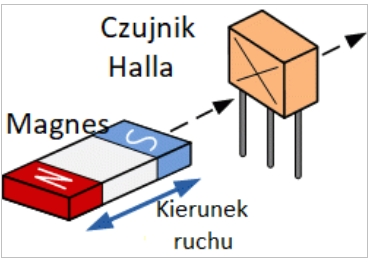
\includegraphics[width=0.5\textwidth]{./graf/halla-enc.jpg}
    \caption{Rysunek przedstawiający zasadę działania czujnika Hall'a \cite{bib:hall_net}}
    \label{rys2:encoders-graf}
\end{figure}

\subsection{Enkodery kwadraturowe}

Enkodery kwadraturowe to specjalny rodzaj enkoderów, które umożliwiają nie tylko pomiar prędkości i położenia, ale także kierunku obrotu. Składają się z dwóch sygnałów wyjściowych – A i B – przesuniętych względem siebie o fazę 90°. Dzięki temu fazowemu przesunięciu system sterujący jest w stanie określić kierunek obrotu, analizując, który z sygnałów A lub B wyprzedza drugi. Każdy impuls generowany przez sygnały A i B odpowiada określonemu przemieszczeniu kątowemu, co pozwala na wyznaczenie pozycji kątowej osi obrotu z wysoką precyzją.


\begin{figure}[h]
    \centering
    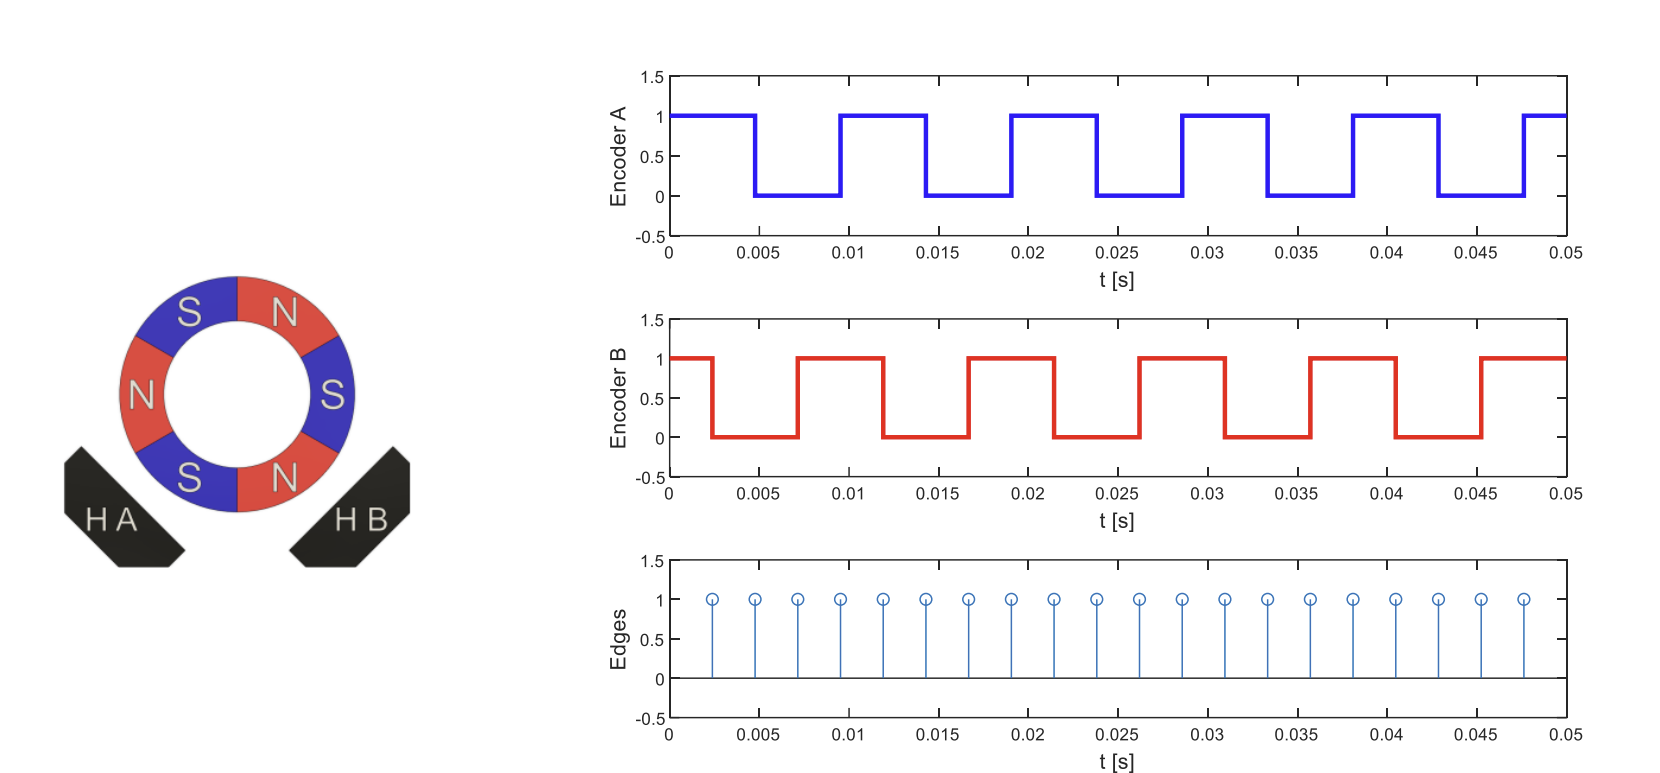
\includegraphics[width=0.8\textwidth]{./graf/enkoders.png}
    \caption{Rysunek przedstawiający ideowo budowę enkodera kwadraturowego oraz sygnałów przez niego generowanych \cite{bib:encoders-pid}}
    \label{rys2:encoders-graf}
\end{figure}


\begin{figure}[h]
    \centering
    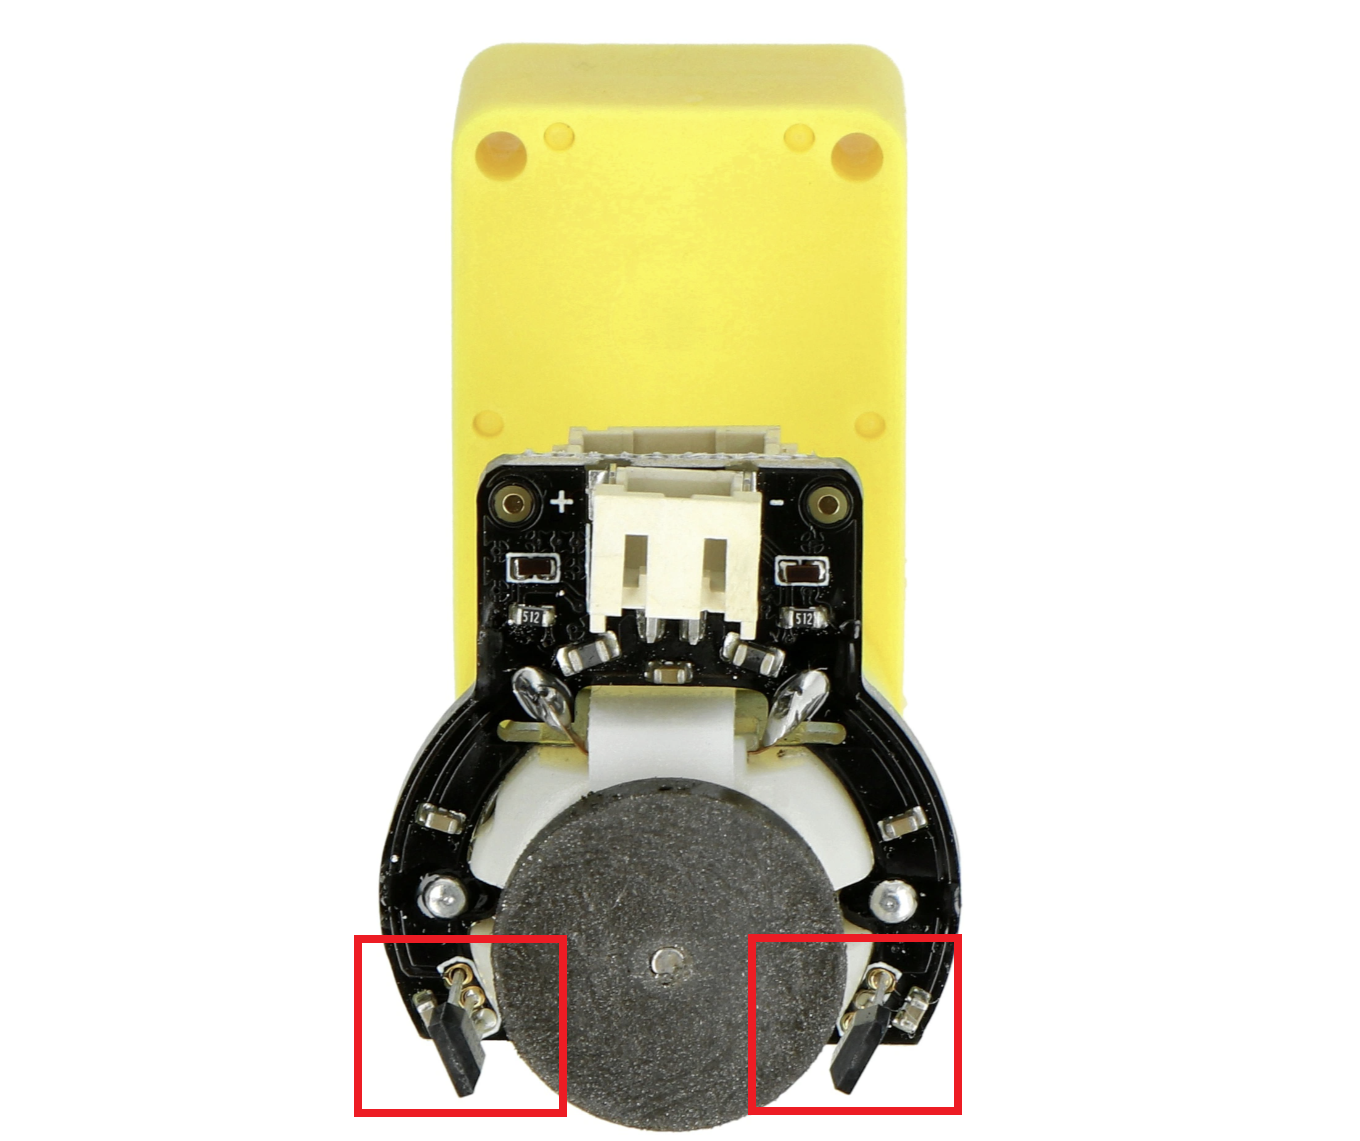
\includegraphics[width=0.5\textwidth]{./graf/enkoder-silnik.png}
    \caption{Rysunek przedstawiający przykładowy wygląd enkodera opartego o efekt Hall'a. Czerwonymi kwadratami są zaznaczone tranzystory wykrywające zmianę pola magnetycznego podczas obrotu wału \cite{bib:botland-hall}}
    \label{rys2:encoders-graf}
\end{figure}

\clearpage

\section{Regulator PID}

Regulator PID (ang. \textit{Proportional-Integral-Derivative}) jest jednym z najczęściej stosowanych regulatorów w systemach automatycznego sterowania, ze względu na swoją prostotę implementacji oraz skuteczność w wielu aplikacjach przemysłowych i robotycznych. Regulator ten wykorzystuje trzy składniki: proporcjonalny, całkujący oraz różniczkujący.

\subsection{Ogólny schemat układu regulacji}

\begin{figure}[h]
    \centering
    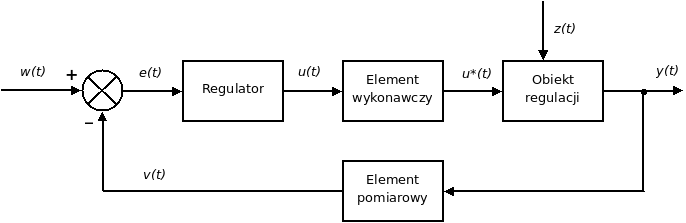
\includegraphics[width=0.5\textwidth]{./graf/regulacja1.png}
    \caption{Rysunek przedstawiający ogólny schemat układu regulacji automatycznej \cite{bib:wiki-regulacja}}
    \label{rys2:regulacja1}
\end{figure}

\subsection{Działanie regulatora PID}

Działanie regulatora PID opiera się na przetwarzaniu sygnału uchybu $e(t)$, czyli różnicy między wartością zadaną $y_{set}$ a wartością rzeczywistą $y(t)$ wielkości regulowanej:

\begin{equation}
e(t) = y_{set} - y(t)
\end{equation}

Regulator PID wyznacza wartość sygnału sterującego $u(t)$ jako sumę trzech składników:
\begin{equation}
u(t) = K_p e(t) + K_i \int_{0}^{t} e(\tau) d\tau + K_d \frac{de(t)}{dt}
\end{equation}
gdzie:
\begin{itemize}
    \item $K_p$ – współczynnik proporcjonalny, który wzmacnia aktualny uchyb,
    \item $K_i$ – współczynnik całkujący, który reaguje na sumę uchybów w czasie,
    \item $K_d$ – współczynnik różniczkujący, który reaguje na zmianę uchybu.
\end{itemize}

Każda ze składowych regulatora PID pełni inną funkcję, a ich kombinacja pozwala na precyzyjne kontrolowanie zachowania systemu.

\subsection{Składnik proporcjonalny $P$}

Składnik proporcjonalny jest liniowo zależny od uchybu $e(t)$ i odpowiada za natychmiastową reakcję na różnicę między wartością zadaną a rzeczywistą. Działa zgodnie ze wzorem:

\begin{equation}
P(t) = K_p e(t)
\end{equation}

Im większa wartość $K_p$, tym regulator bardziej dynamicznie reaguje na uchyb, co może przyspieszyć osiągnięcie wartości zadanej, ale przy zbyt dużych wartościach może prowadzić do przeregulowania lub oscylacji.

\subsection{Składnik całkujący $I$}

Składnik całkujący sumuje uchyby w czasie, co pozwala na eliminację uchybu statycznego – różnicy między wartością rzeczywistą a zadaną, która może utrzymywać się w przypadku stosowania tylko składnika proporcjonalnego. Składnik całkujący jest dany równaniem:

\begin{equation}
I(t) = K_i \int_{0}^{t} e(\tau) d\tau
\end{equation}

Dzięki temu składnikowi, regulator PID potrafi zniwelować długotrwały uchyb, chociaż przy zbyt dużych wartościach $K_i$ może wystąpić zjawisko przeregulowania i niestabilność.

\subsection{Składnik różniczkujący $D$}

Składnik różniczkujący uwzględnia szybkość zmian uchybu $e(t)$, co pozwala na szybsze reagowanie na gwałtowne zmiany i przeciwdziałanie efektowi przeregulowania. Opisuje go wyrażenie:

\begin{equation}
D(t) = K_d \frac{de(t)}{dt}
\end{equation}

Ten składnik regulatora poprawia stabilność i tłumi oscylacje, jednak zbyt duża wartość $K_d$ może prowadzić do niestabilności układu, zwłaszcza w obecności szumów.

\subsection{Pełne równanie regulatora PID}

Łącząc wszystkie trzy składniki, równanie regulatora PID przyjmuje postać:

\begin{equation}
u(t) = K_p e(t) + K_i \int_{0}^{t} e(\tau) d\tau + K_d \frac{de(t)}{dt}
\end{equation}

gdzie:
\begin{itemize}
    \item $K_p e(t)$ – składnik proporcjonalny, który odpowiada za szybką reakcję na zmiany,
    \item $K_i \int_{0}^{t} e(\tau) d\tau$ – składnik całkujący, który eliminuje uchyb statyczny,
    \item $K_d \frac{de(t)}{dt}$ – składnik różniczkujący, który przeciwdziała nagłym zmianom uchybu.
\end{itemize}

Regulacja parametrów $K_p$, $K_i$ i $K_d$ pozwala na dostosowanie charakterystyki regulatora PID do specyfiki sterowanego obiektu. Optymalne wartości tych parametrów zazwyczaj są dobierane metodą prób i błędów lub za pomocą metod takich jak strojenie Zieglera-Nicholsa.

\subsection{Zastosowanie regulatora PID w sterowaniu robotem mobilnym}

W omawianym projekcie regulator PID znajduje zastosowanie w kontrolowaniu odległości jaką pokonuje platforma mobilna poprzez odpowiednie sterowanie napięciem zasilania elementów wykonawczych. Nastawy regulatora zostały dostosowane metodą prób i błędów z racji trdudnego do zamodelowania układu dynamicznego. Uzyskana jakość regulacji jest wystarczająca do spełnienia wymagań projektowych. 

\section{Podstawy wykrywania krawędzi w wizji komputerowej}

Wykrywanie krawędzi stanowi kluczowy element analizy obrazów w kontekście wizji komputerowej. Jest to technika mająca na celu identyfikację istotnych zmian w intensywności pikseli obrazu, które zazwyczaj wskazują na obecność krawędzi obiektów. Krawędzie odgrywają fundamentalną rolę w percepcji kształtów i struktur, dlatego ich wykrywanie jest podstawą wielu aplikacji, takich jak segmentacja obrazu, rozpoznawanie obiektów oraz analiza ruchu.

Jedną z najbardziej popularnych metod wykrywania krawędzi jest algorytm Canny’ego, który został zaproponowany przez Johna F. Canny'ego w 1986 roku. Metoda ta jest ceniona za swoją zdolność do wydobywania krawędzi z obrazów przy jednoczesnym zachowaniu ich jakości oraz redukcji szumów.

\subsection{Algorytm Canny’ego}

Algorytm Canny’ego składa się z kilku kluczowych kroków:

1. \textbf{Wygładzenie} (ang. \english{Smoothing}): Na początku obraz poddawany jest filtracji w celu zredukowania szumów. Zazwyczaj stosuje się filtr Gaussa, który jest reprezentowany przez macierz:

\[
G = \begin{bmatrix}
\frac{1}{16} & \frac{1}{8} & \frac{1}{16} \\
\frac{1}{8} & \frac{1}{4} & \frac{1}{8} \\
\frac{1}{16} & \frac{1}{8} & \frac{1}{16}
\end{bmatrix}
\]

2. \textbf{Obliczenie gradientu:} Następnie obliczane są gradienty obrazu, aby zidentyfikować kierunki zmian intensywności. Używa się do tego macierzy \textit{Sobela}, które pozwalają na obliczenie gradientu w kierunkach poziomym (Gx) i pionowym (Gy):

\[
S_x = \begin{bmatrix}
-1 & 0 & 1 \\
-2 & 0 & 2 \\
-1 & 0 & 1
\end{bmatrix}, \quad 
S_y = \begin{bmatrix}
1 & 2 & 1 \\
0 & 0 & 0 \\
-1 & -2 & -1
\end{bmatrix}
\]

Gradient można obliczyć jako:

\[
G = \sqrt{G_x^2 + G_y^2}
\]
oraz jego kierunek:

\[
\Theta = \text{atan2}(G_y, G_x)
\]

3. \textbf{Tłumienie nie-maksymalne} (ang. \english{Non-maximum suppression}): W kolejnym kroku następuje eliminacja pikseli, które nie są lokalnymi maksimami w kierunku gradientu, co pozwala na wyostrzenie krawędzi.

4. \textbf{Podwójne progowanie} (ang. \english{Double thresholding}): Algorytm wprowadza dwa progi: wysoki i niski. Piksele, które przekraczają wysoki próg, są uznawane za krawędzie, natomiast te, które są poniżej niskiego progu, są odrzucane. Piksele, które mieszczą się między tymi dwoma progami, są klasyfikowane jako krawędzie słabe.

5. \textbf{Śledenie krawędzi z histerezą} (ang. \english{Edge tracking by hysteresis}): Ostatnim krokiem jest śledzenie krawędzi, gdzie słabe krawędzie są zachowywane, jeśli są połączone z mocnymi krawędziami. To pozwala na eliminację przypadkowych detekcji krawędzi i zapewnia spójność wyników.

\clearpage

\section{Podstawy rozpoznawania kolorów w wizji komputerowej}

Rozpoznawanie kolorów w wizji komputerowej to kluczowy aspekt w wielu aplikacjach automatyki, robotyki oraz sztucznej inteligencji. W kontekście robotyki, techniki te pozwalają na identyfikację i klasyfikację obiektów w otoczeniu robota, co jest istotne dla jego nawigacji oraz interakcji z otoczeniem. W niniejszej sekcji omówione zostaną podstawowe zasady oraz techniki wykorzystywane w procesie rozpoznawania kolorów.

\subsection{Teoria koloru}


Kolor jest percepcją widzialnego spektrum światła, które jest odbierane przez ludzkie oczy i interpretowane przez mózg. W wizji komputerowej kolory są często reprezentowane za pomocą różnych modeli kolorów, w tym w przestrzeni kolorów RGB (ang. \english{Red, Green, Blue}) \textit{rys.} [\ref{rys2:rgb1}], HSV (ang. \english{Hue, Saturation, Value}) \textit{rys.} [\ref{rys2:hsv1}] oraz YCrCb (ang. \english{Luminance, Chrominance}) \textit{rys.} [\ref{rys2:ycrcb1}]. W modelu RGB kolory są definiowane przez intensywności trzech składowych kolorów, podczas gdy w modelu HSV kolory są określane na podstawie ich odcienia, nasycenia i jasności, co ułatwia przetwarzanie i rozpoznawanie kolorów w kontekście wizji komputerowej. Model YCrCb, z kolei, oddziela informację o luminancji (jasności) od informacji o chrominancji (kolorze), co jest szczególnie przydatne w kompresji obrazów oraz w systemach wizyjnych, umożliwiając efektywną analizę kolorów przy jednoczesnym zredukowaniu wpływu zmian oświetleniowych.


\begin{figure}[H]
    \centering
    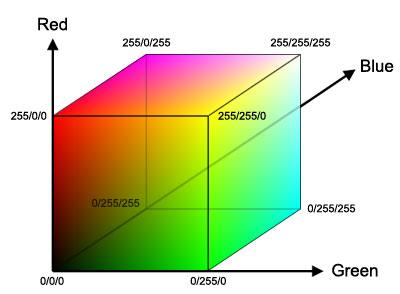
\includegraphics[width=0.6\textwidth]{./graf/rgb-model.png}
    \caption{Rysunek przedstawiający wizualizację przestrzeni kolorów RGB \cite{bib:rgb-model}}
    \label{rys2:rgb1}
\end{figure}

\begin{figure}[h]
    \centering
    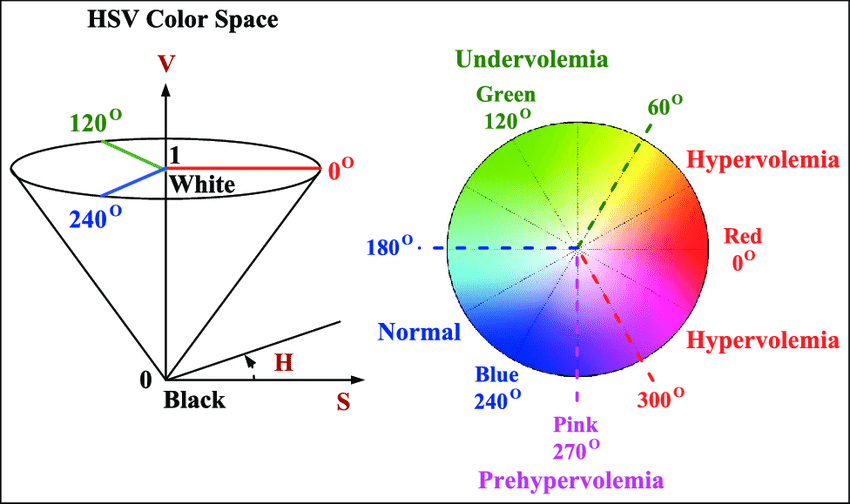
\includegraphics[width=0.6\textwidth]{./graf/hsv-model.png}
    \caption{Rysunek przedstawiający wizualizację przestrzeni HSV \cite{bib:hsv-model}}
    \label{rys2:hsv1}
\end{figure}


\begin{figure}[h]
    \centering
    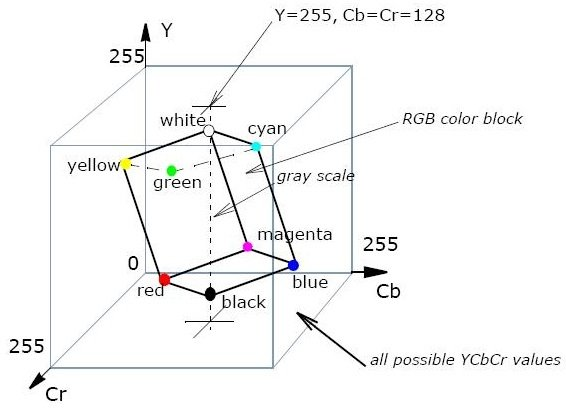
\includegraphics[width=0.6\textwidth]{./graf/ycrcb-model.png}
    \caption{Rysunek przedstawiający wizualizację przestrzeni YCrCb \cite{bib:ycrcb-model}}
    \label{rys2:ycrcb1}
\end{figure}

\clearpage

\subsection{Proces rozpoznawania kolorów}

Proces rozpoznawania kolorów w obrazach polega na identyfikacji oraz klasyfikacji pikseli na podstawie ich wartości kolorystycznych. Kluczowe etapy tego procesu obejmują:

\begin{enumerate}
    \item \textbf{Przechwytywanie obrazu:} Obraz jest przechwytywany za pomocą kamery cyfrowej, która generuje dane w formacie cyfrowym. 
    \item \textbf{Przetwarzanie obrazu:} Na tym etapie obraz jest poddawany różnym operacjom, takim jak filtracja, segmentacja i transformacja kolorów, aby wyodrębnić istotne informacje. 
    \item \textbf{Ekstrakcja cech:} Następnie przeprowadzana jest analiza danych kolorystycznych w celu identyfikacji i klasyfikacji obiektów na podstawie ich kolorów. 
    \item \textbf{Decyzja:} Na końcu system podejmuje decyzje o klasifikacji obiektów bazując na wcześniej zebranych informacjach o kolorze.
\end{enumerate}

\subsection{Algorytmy rozpoznawania kolorów}

W literaturze przedmiotu opisano wiele algorytmów wykorzystywanych w rozpoznawaniu kolorów, w tym metody oparte na histogramie, segmentacji obrazu oraz analizy cech. Histogramy kolorów są popularnym narzędziem do analizy rozkładu kolorów w obrazie, co pozwala na szybką identyfikację dominujących kolorów.

Segmentacja obrazu to proces dzielenia obrazu na różne regiony na podstawie ich kolorów, co ułatwia identyfikację obiektów w danym kolorze. Algorytmy takie jak k-means clustering czy metoda watershed są często stosowane w celu wydzielenia obiektów o określonym kolorze z tła.

DO POPRAWY - TRZEBA DO JESZCZE SENSOWNIE OPISAĆ (!!!!) % [Właściwy dla kierunku -- np. Specyfikacja zewnętrzna]

% TODO
\chapter{[Właściwy dla kierunku -- np. Specyfikacja wewnętrzna]}
\label{ch:05}


Jeśli „Specyfikacja wewnętrzna”:
\begin{itemize}
\item przedstawienie idei
\item architektura systemu
\item opis struktur danych (i organizacji baz danych)
\item komponenty, moduły, biblioteki, przegląd ważniejszych klas (jeśli występują)
\item przegląd ważniejszych algorytmów (jeśli występują)
\item szczegóły implementacji wybranych fragmentów, zastosowane wzorce projektowe
\item diagramy UML
\end{itemize}

% % % % % % % % % % % % % % % % % % % % % % % % % % % % % % % % % % % 
% Pakiet minted wymaga importu: \usepackage{minted}                 %
% i specjalnego kompilowania:                                       %
% pdflatex -shell-escape main                                       %
% % % % % % % % % % % % % % % % % % % % % % % % % % % % % % % % % % % 


Krótka wstawka kodu w linii tekstu jest możliwa, np.  \lstinline|int a;| (biblioteka \texttt{listings})% lub  \mintinline{C++}|int a;| (biblioteka \texttt{minted})
. 
Dłuższe fragmenty lepiej jest umieszczać jako rysunek, np. kod na rys \ref{fig:pseudokod:listings}% i rys. \ref{fig:pseudokod:minted}
, a naprawdę długie fragmenty – w załączniku.


\begin{figure}
\centering
\begin{lstlisting}
class test : public basic
{
    public:
      test (int a);
      friend std::ostream operator<<(std::ostream & s, 
                                     const test & t);
    protected:
      int _a;  
      
};
\end{lstlisting}
\caption{Pseudokod w \texttt{listings}.}
\label{fig:pseudokod:listings}
\end{figure}

%\begin{figure}
%\centering
%\begin{minted}[linenos,frame=lines]{c++}
%class test : public basic
%{
%    public:
%      test (int a);
%      friend std::ostream operator<<(std::ostream & s, 
%                                     const test & t);
%    protected:
%      int _a;  
%      
%};
%\end{minted}
%\caption{Pseudokod w \texttt{minted}.}
%\label{fig:pseudokod:minted}
%\end{figure}


 % [Właściwy dla kierunku -- np. Specyfikacja wewnętrzna]

% TODO
\chapter{Specyfikacja techniczna}
\label{ch:06}

\section{Konstrukcja}
Proces konstrukcji robota przebiegał w dwóch głównych etapach. Pierwszy z nich miał na celu przygotowanie prototypowej wersji robota, która spełnia podstawowe wymagania wynikające z założeń konstrukcyjnych dotyczących napędu oraz sterowania. Drugi etap opiewał na wykonanie pełnego projektu robota w programie Autodesk Fusion 360, spełniającego wszystkie techniczne wymogi projektu, z bardzo dobrą dokładnością, w celu wyeliminowania błędów wynikających z konstrukcji mechanicznej.

\subsection{Pierwsza wersja konstrukcji}

W fazie prototypowej zdecydowano się na wykorzystanie sklejki brzozowej – materiału taniego, lekkiego oraz łatwego w obróbce. Platforma bazowa prototypu miała wymiary: 240 mm długości oraz 220 mm szerokości. Silniki zostały osadzone na osi poprzecznej robota, zgodnie z wymogami nakładanymi przez sposób napędu. 

Taka konfiguracja umożliwiła szybką weryfikację działania elementów wykonawczych oraz systemu sterowania, jeszcze przed przystąpieniem do bardziej zaawansowanych prac konstrukcyjnych. Zdjęcie [\ref{zdj:prototyp}] przedstawia opisany prototyp. 

\hspace{1cm}

W toku prac nad wczesną wersją, po osiągnięciu zadowalającej precyzji sterowania, do konstrukcji dołączono przednią ścianę, do której przymocowano chwytak [\ref{zdj:prototyp-chwytak}]. Umożliwiło to przetestowanie poprawności działania wszystkich elementów wykonawczych obecnych na platformie mobilnej. Dodatkowo, równocześnie przeprowadzono testy pełnej komunikacji między kontrolerem silników a komputerem Raspberry Pi, który pełnił rolę głównej jednostki obliczeniowej robota. W tym kroku zweryfikowano, czy platforma poprawnie reaguje na przesyłane komendy oraz czy nie występują żadne błędy w komunikacji lub wykonaniu poleceń.

% \begin{figure}[h!]
%   \centering
%   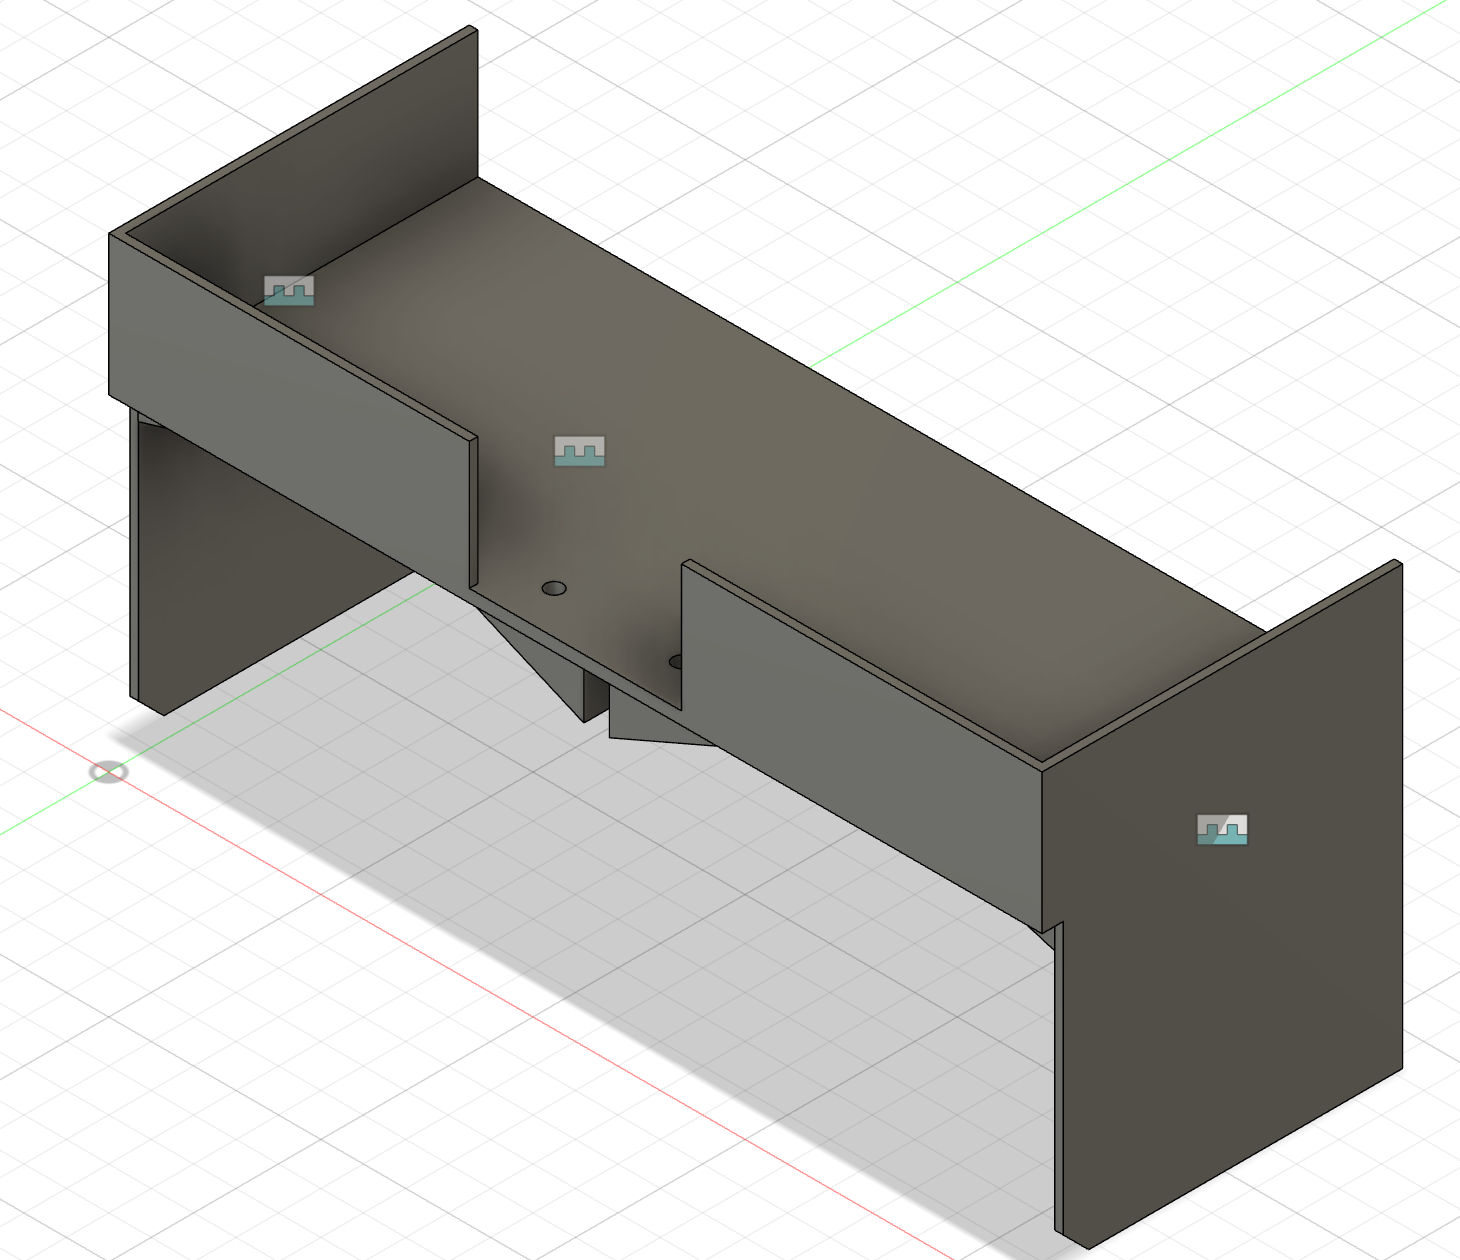
\includegraphics[width=0.7\textwidth]{./graf/upper.png}
%   \caption{Model górnej części obudowy}
%   \label{fig:ball-close}
% \end{figure}

% \begin{figure}[h!]
%   \centering
%   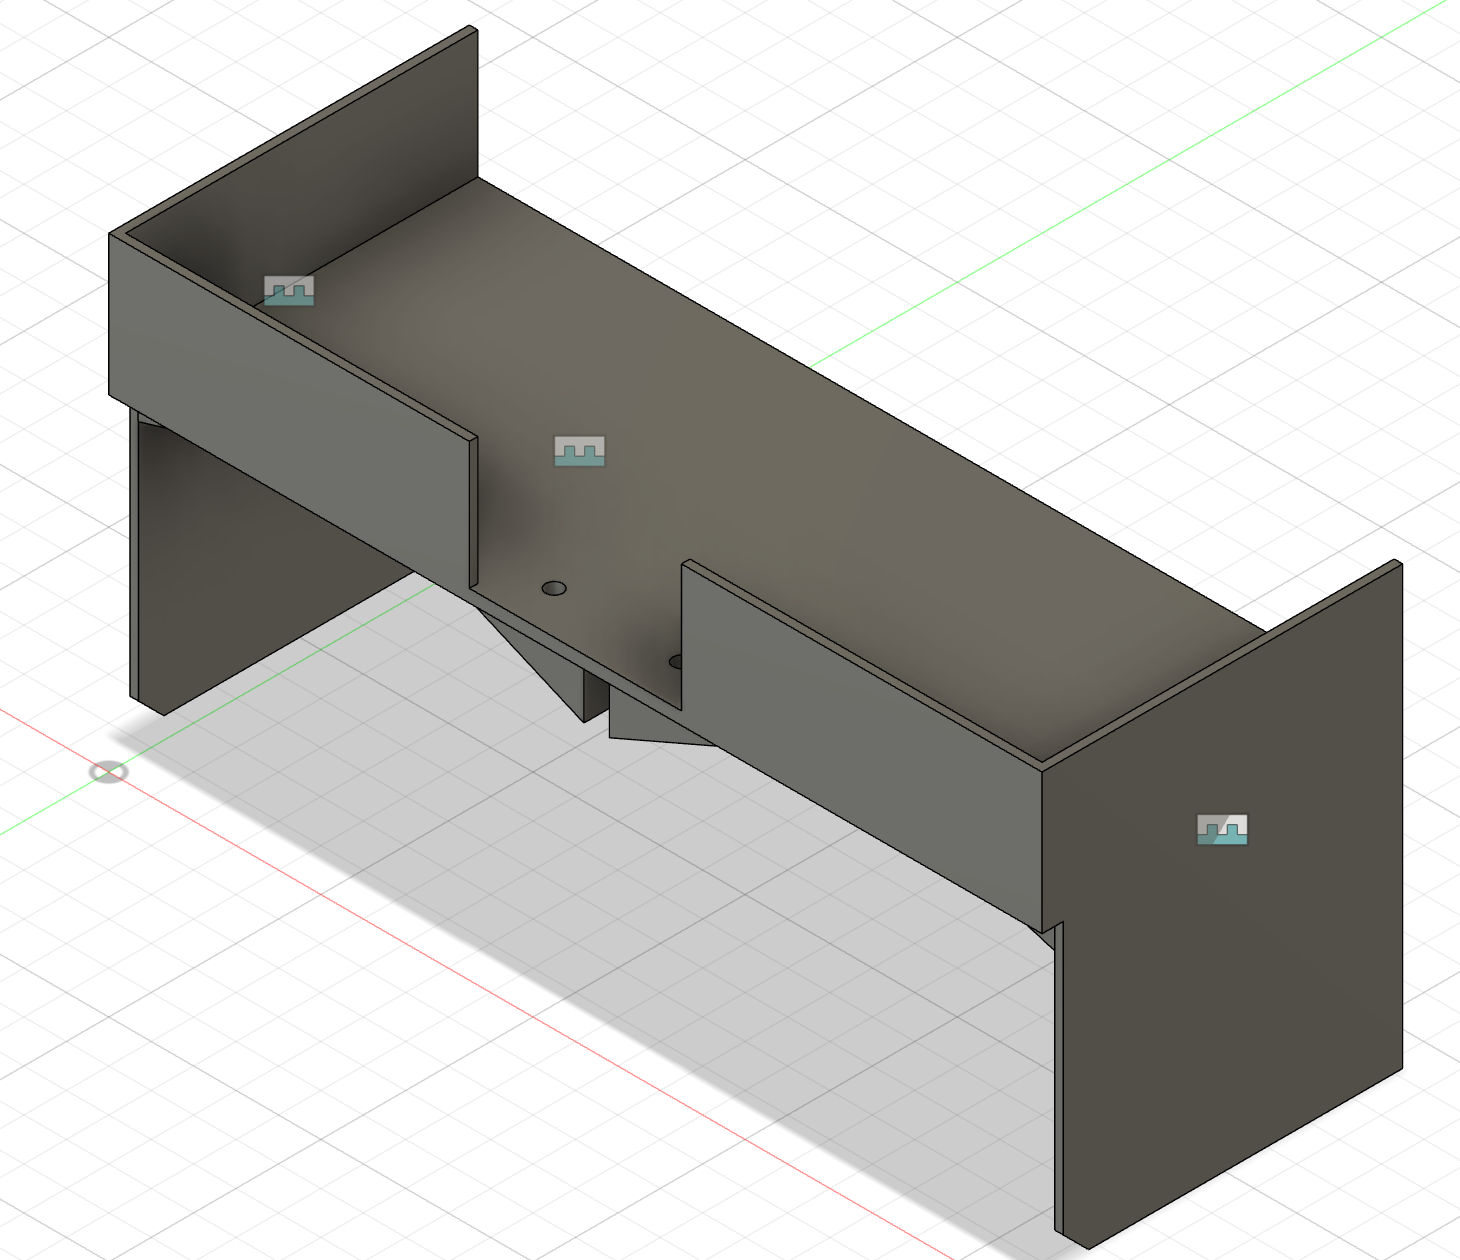
\includegraphics[width=0.7\textwidth]{./graf/upper.png}
%   \caption{Model górnej części obudowy}
%   \label{fig:ball-close}
% \end{figure}

\subsection{Właściwy projekt robota mobilnego}

Po pozytywnym zakończeniu walidacji funkcjonowania algorytmów sterowania i komunikacji, przystąpiono do drugiego etapu konstrukcji – zaprojektowania i wytworzenia docelowej obudowy bazowej robota. Obudowa została wykonana przy użyciu technologii druku 3D, co pozwoliło na uzyskanie wysokiej precyzji oraz wprowadzeniu niezbędnych modyfikacji konstrukcyjnych w stosunku do prototypu. Ze względu na ograniczenia przestrzeni roboczej urządzenia drukującego, wymiary podstawy platformy zostały przeniesione na plan kwadratu o boku 220 mm.
Przednia ściana została zaprojektowana jako część podłogi, w celu zwiększenia sztywności konstrukcji. Najcięższym elementem całego robota jest chwytak wraz z serwomechanizmem, przez co wytrzymałość przedniej ściany oraz podłogi była kluczowa. Zgodnie z osią do wewnątrz robota została poprowadzona przegroda, pełniąca funkcję podpory dla górnej części platformy.
Finalny projekt podstawy, przygotowany w programie Autodesk Fusion 360, został przedstawiony na rysunku [\ref{fig:full}].

\hspace{1cm} 

Ostatni etap obejmował zaprojektowanie górnej części obudowy, na której zostanie osadzony komputer Raspberry Pi oraz przymocowany uchwyt na kamerę. Sposób osadzenia górnej części na dolnym segmencie opiera się na precyzyjnie wykonanej przerwie, w którą wsuwa się wspornik bazy. Dzięki takiemu rozwiązaniu, w prosty i szybki sposób można zdjąć górną część i dokonać potrzebnych zmian lub modyfikacji. Te atrybuty są szczególnie przydatne podczas fazy testów i ciągłego ulepszania robota.

W wersji docelowej, przeznaczonej do komercyjnego użytkowania, omawiane mocowanie zostałoby zastąpione przez standardowe połączenia śrubowe lub sklejenie, co zwiększyłoby trwałość obudowy.

\hspace{1cm}

Ostateczna wersja platformy mobilnej została zaprezentowana na zdjęciu [\ref{fig:base-full}] oraz jest widoczna na nagraniach załączonych do pracy. Model obudowy stanowi w pełni funkcjonalny, zgodny z założeniami, robot, jednak część mocowań w wersji przeznaczonej do sprzedaży należy zmienić. 

W tym celu zastosowano mocowania, umożliwiające łatwe zdejmowanie i zakładanie górnej części obudowy na podstawę, co znacząco ułatwia konserwację oraz serwisowanie wewnętrznych komponentów.

Finalna wersja platformy mobilnej została zaprezentowana na ilustracji \ref{fig:full}, a także na załączonych nagraniach.


\begin{figure}[H]
  \centering
  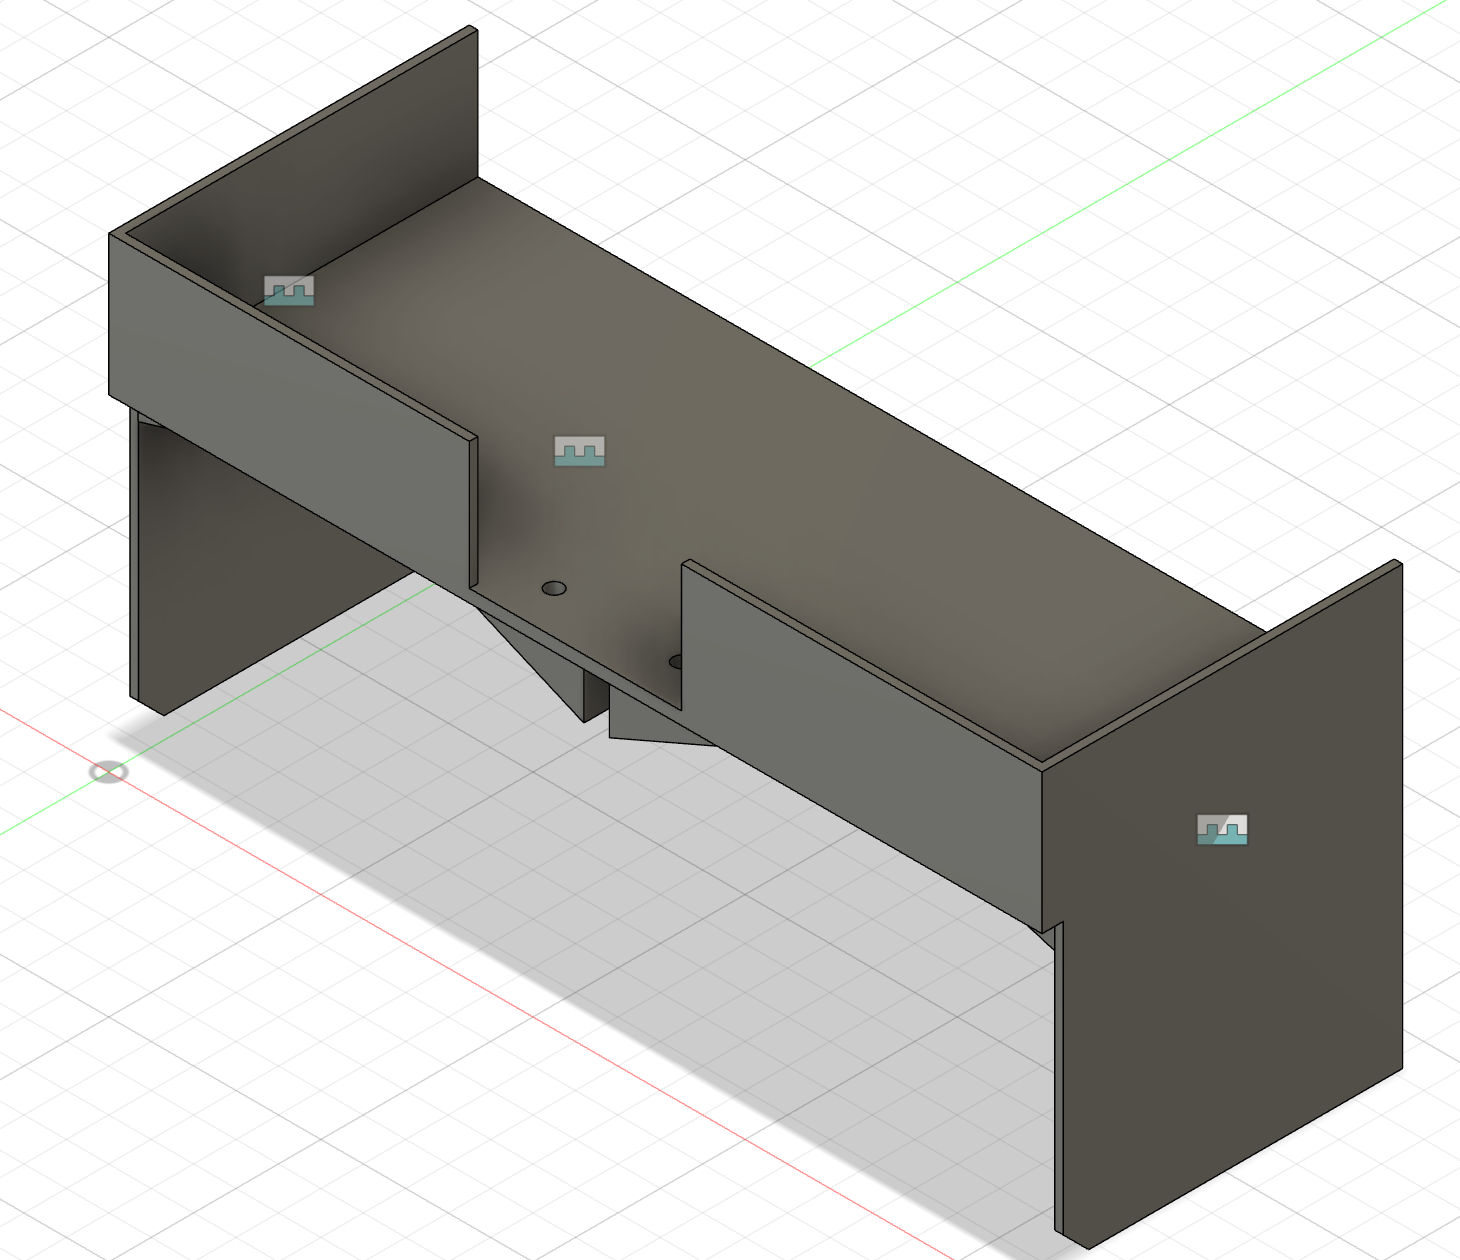
\includegraphics[width=0.7\textwidth]{./graf/upper.png}
  \caption{Model górnej części obudowy}
  \label{fig:ball-close}
\end{figure}

\begin{figure}[H]
  \centering
  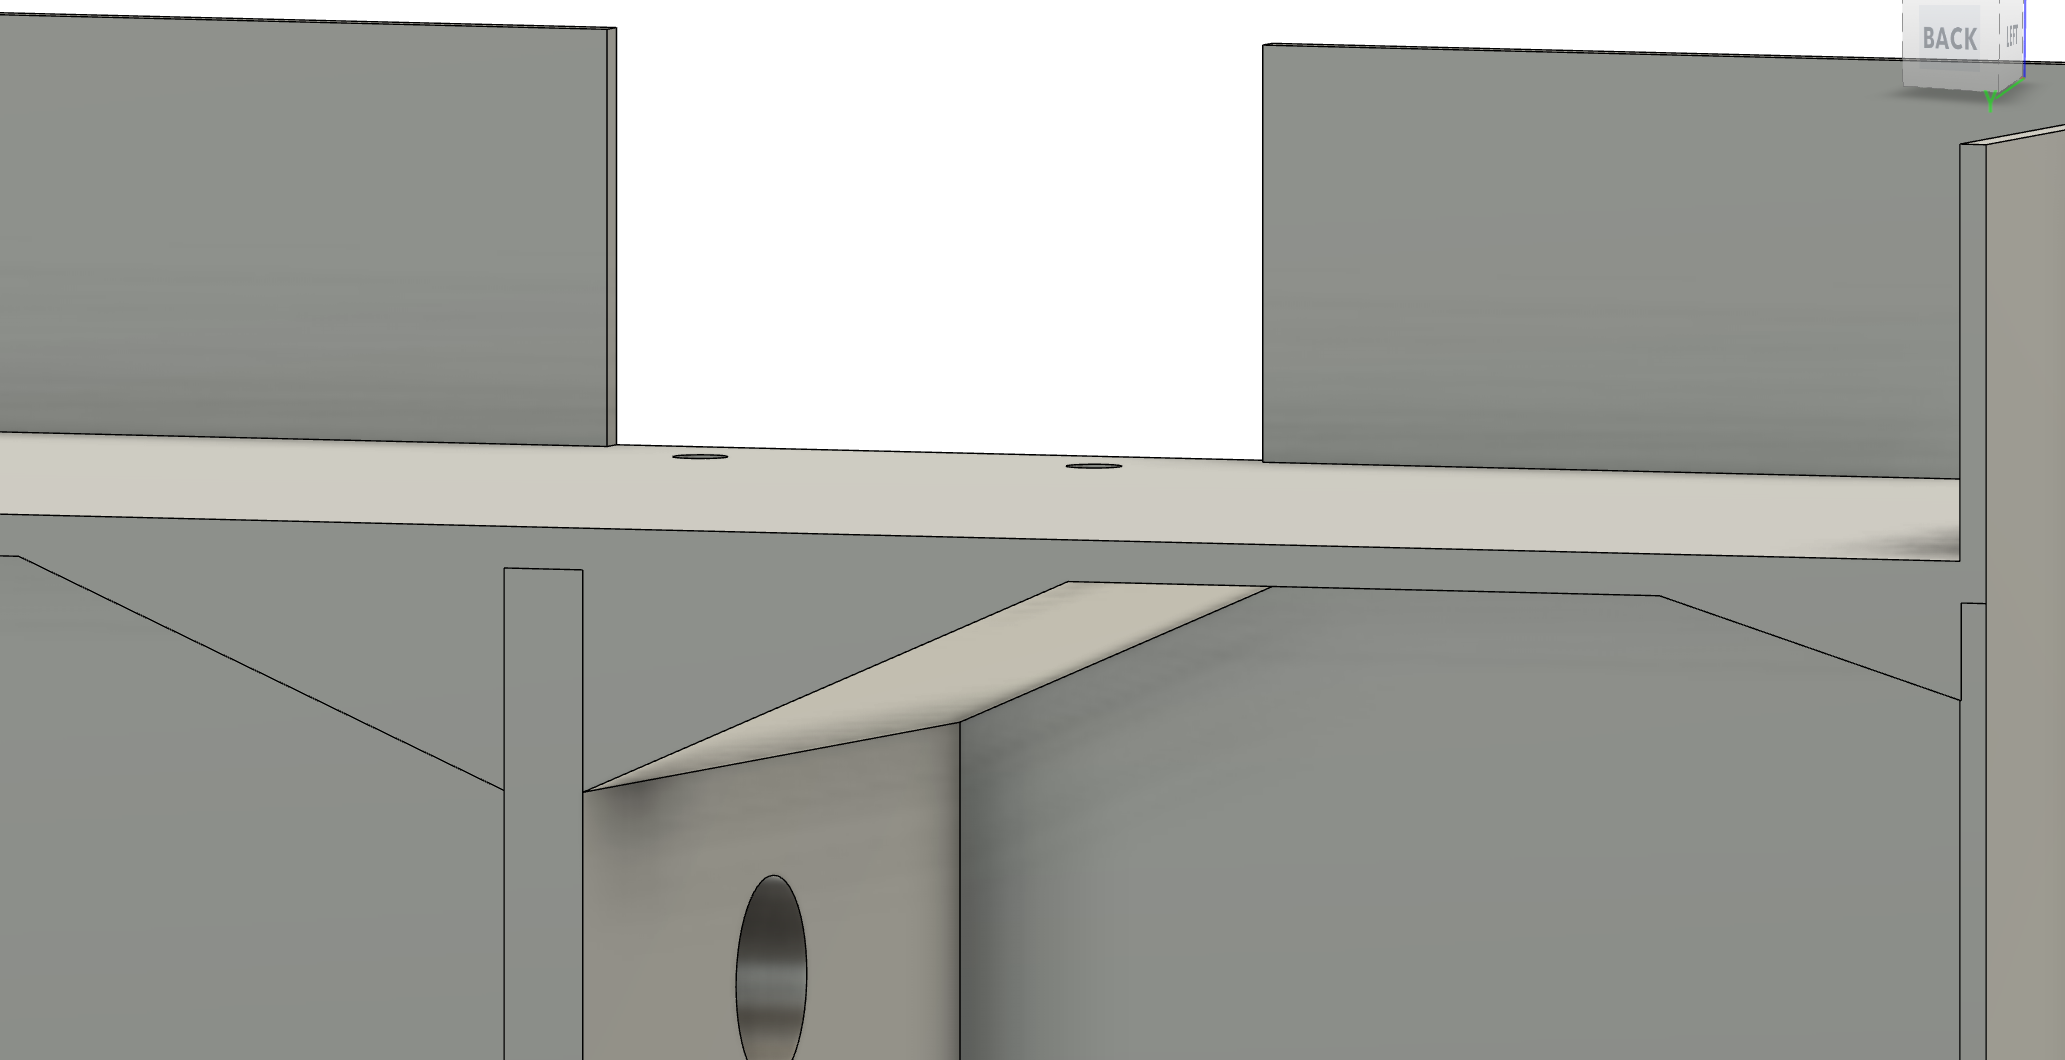
\includegraphics[width=0.7\textwidth]{./graf/full-close.png}
  \caption{Przybliżenie sposobu połączenia górnej części obudowy z dolną. Widoczny jest również otwór przeznaczony na przewody połączeniowe}
  \label{fig:full-close}
\end{figure}


\begin{figure}[H]
  \centering
  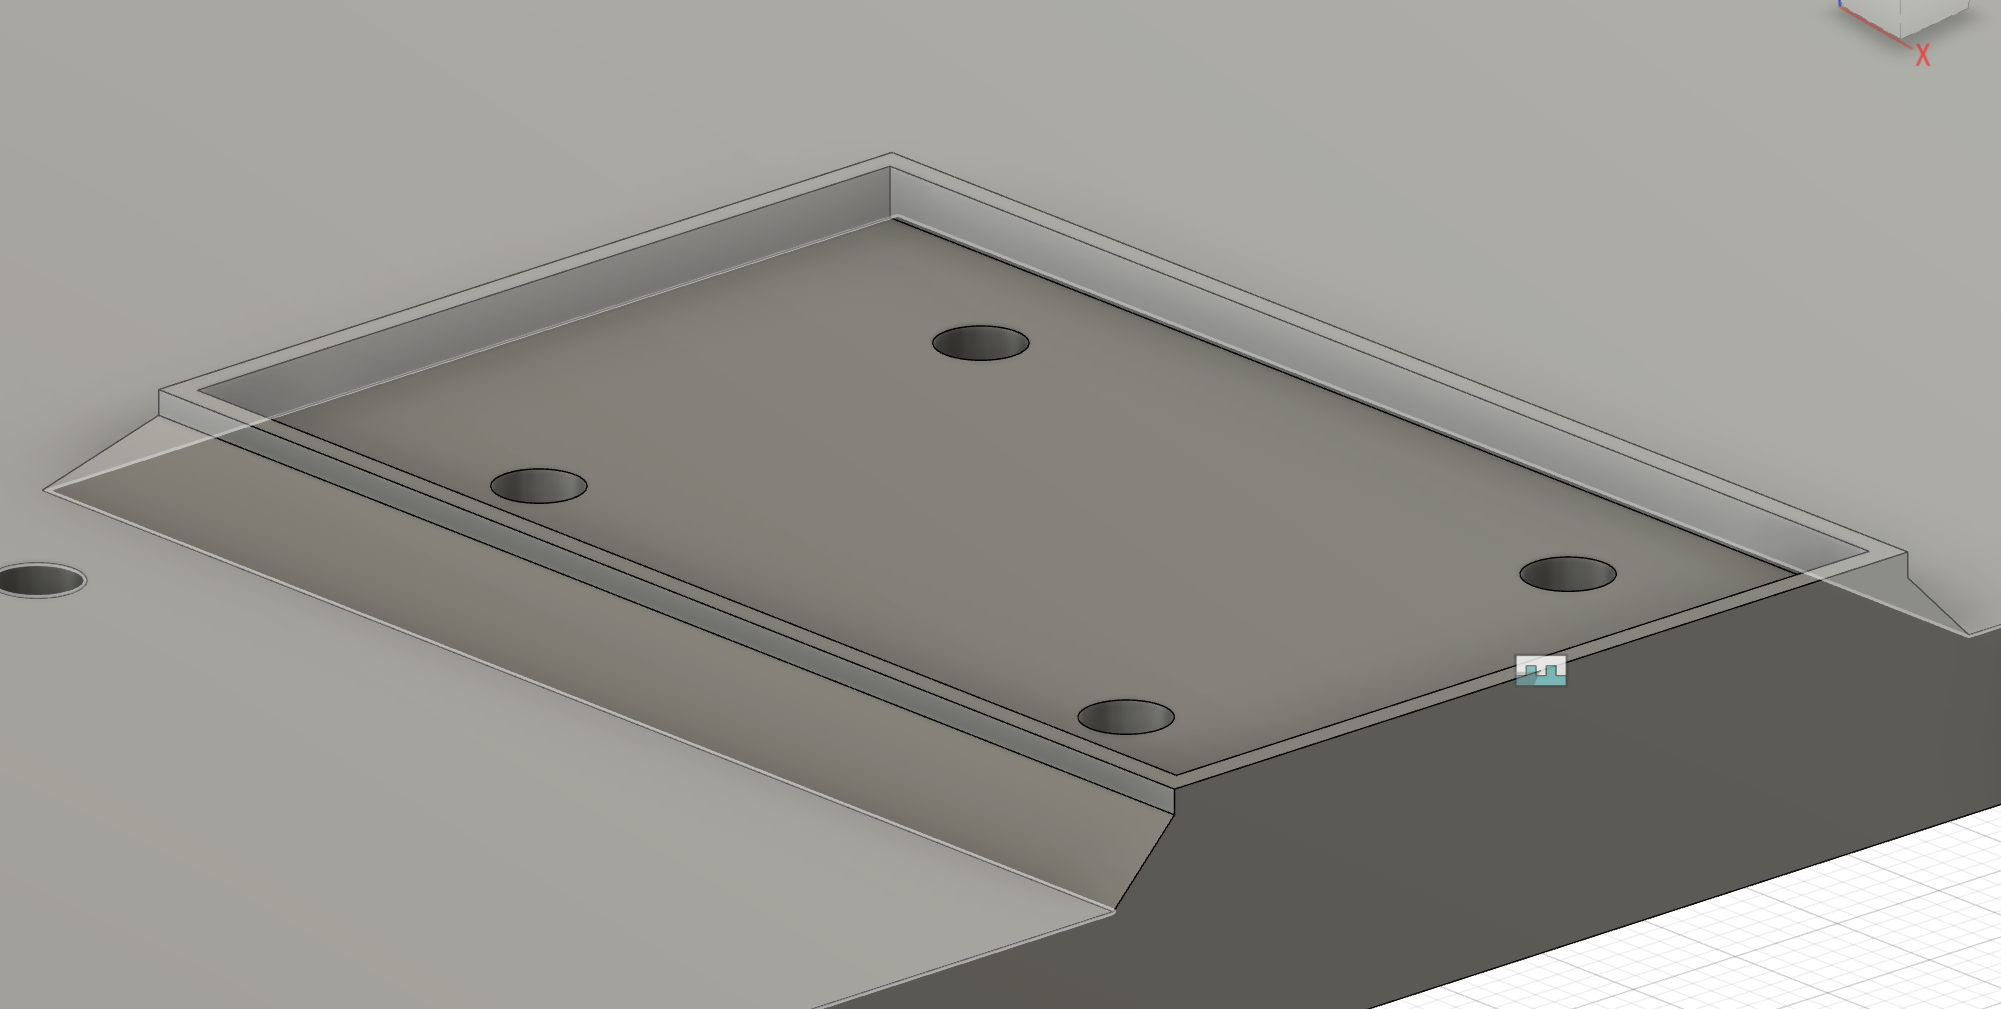
\includegraphics[width=0.5\textwidth]{./graf/motor-close.png}
  \caption{Przybliżenie miejsca na mocowania silników}
  \label{fig:base-close}
\end{figure}

\begin{figure}[H]
  \centering
  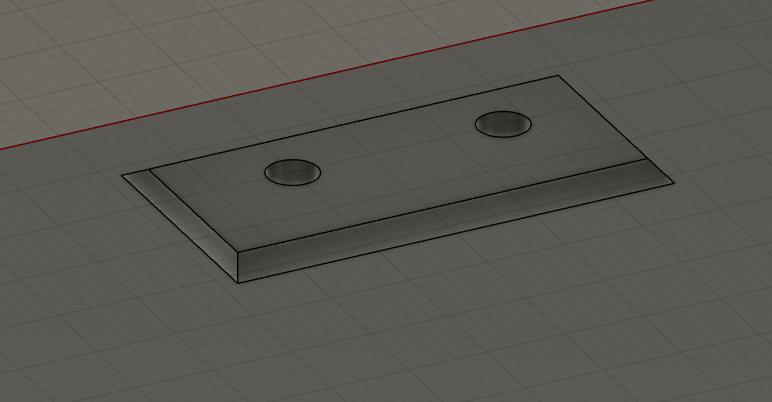
\includegraphics[width=0.5\textwidth]{./graf/ball-close.png}
  \caption{Przybliżenie miejsca mocowania kulek podporowych w osi robota}
  \label{fig:ball-close}
\end{figure}

\begin{figure}[H]
  \centering
  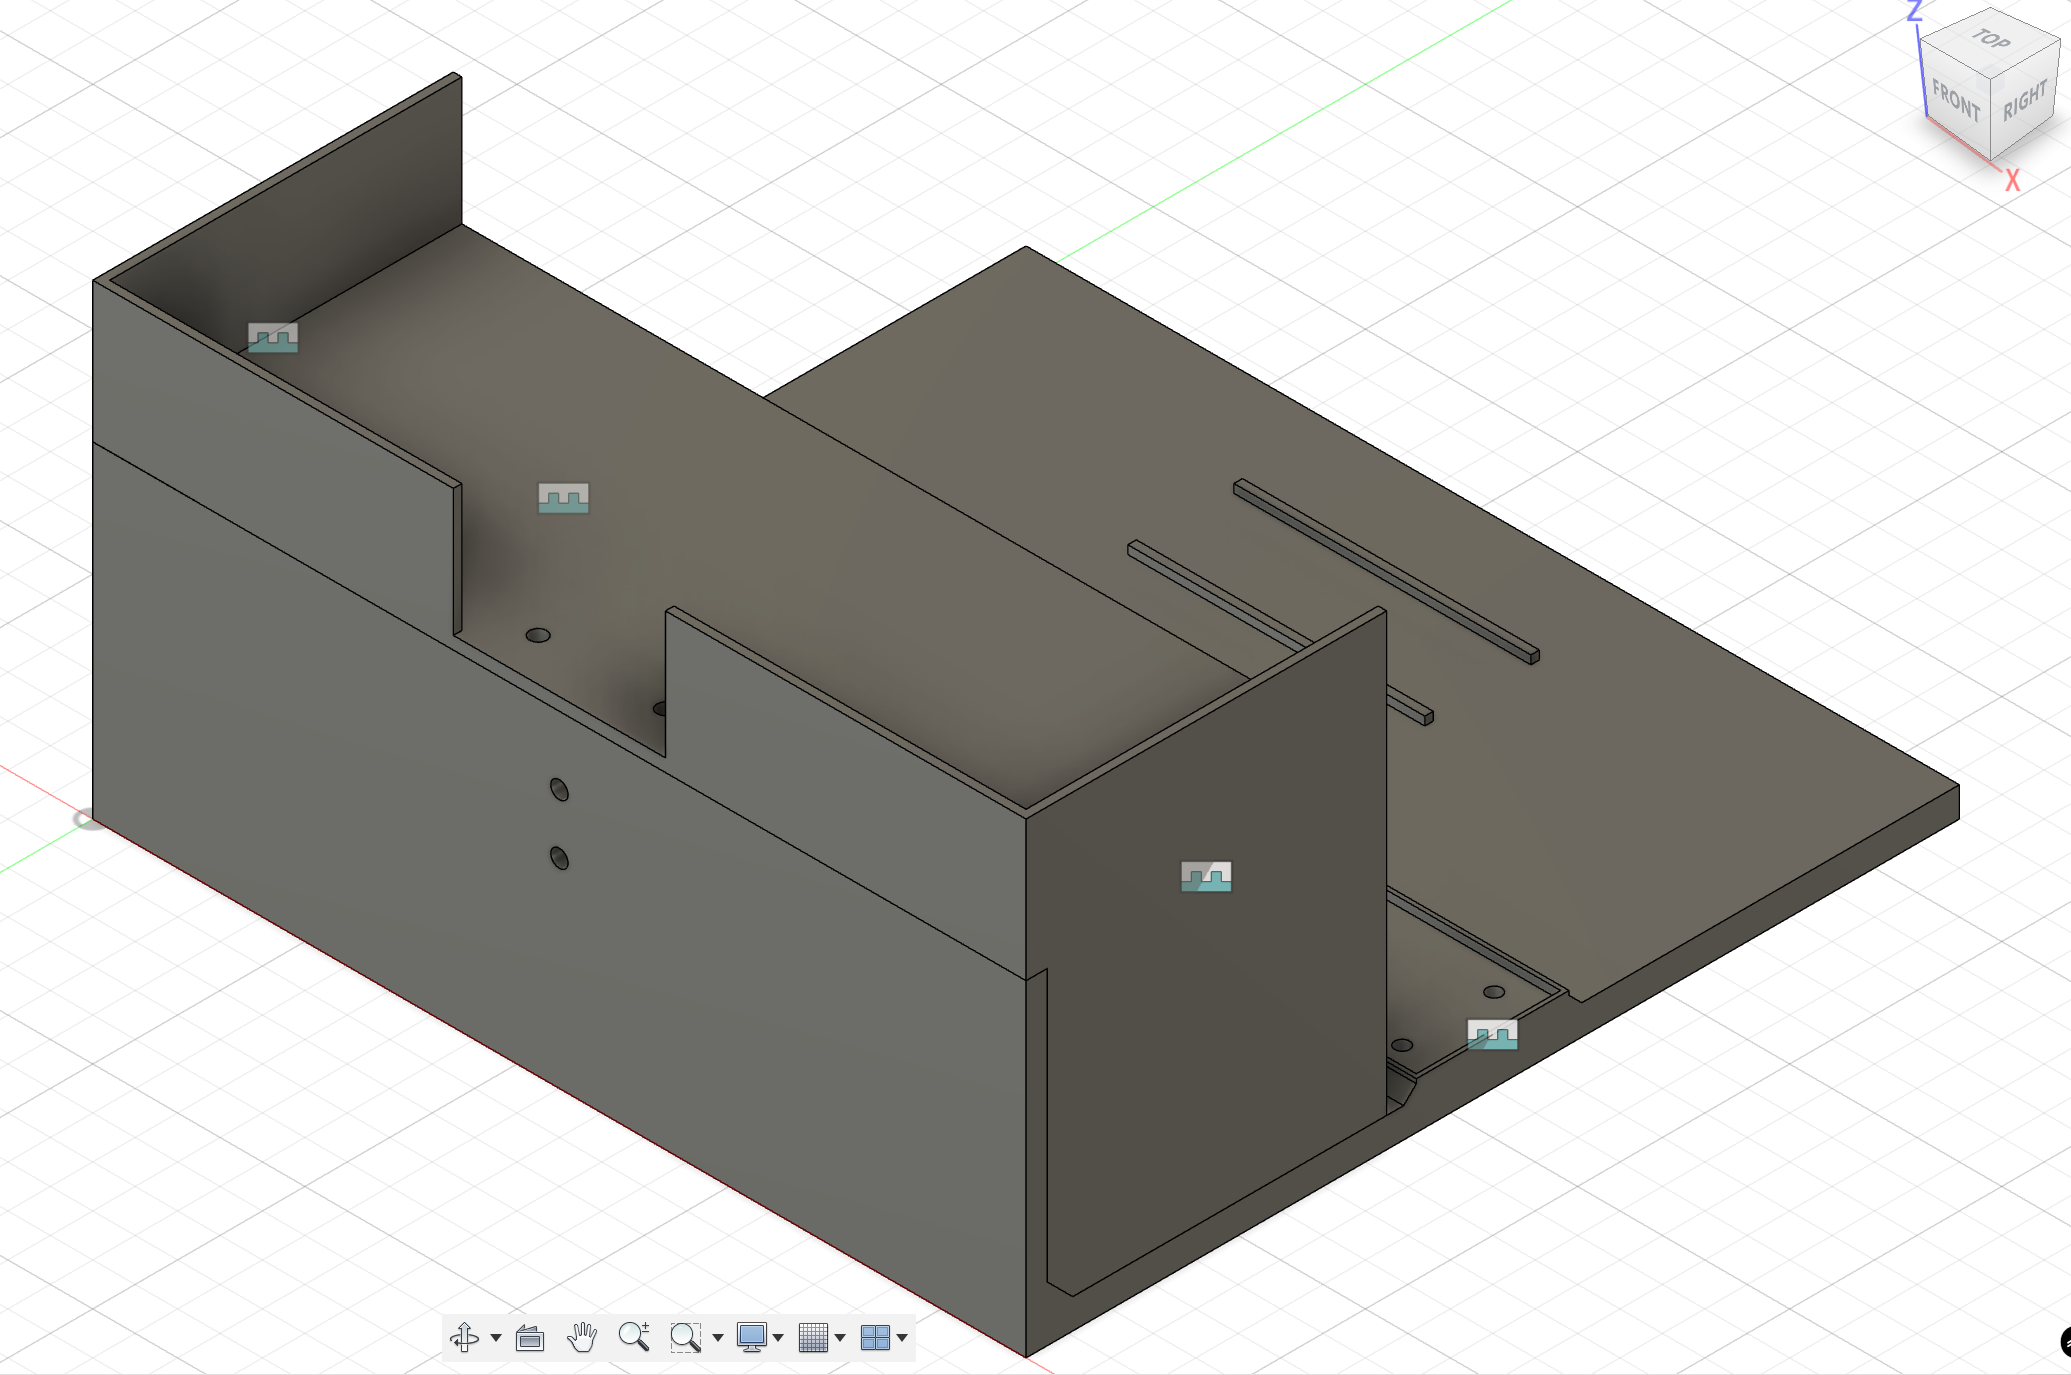
\includegraphics[width=0.9\textwidth]{./graf/full.png}
  \caption{Prezentacja finalnej wersji obudowy robota}
  \label{fig:full}
\end{figure}
 
\clearpage

\section{Implementacja kontrolera silników}

Aplikacja kontrolera silników została zaimplementowana w środowisku Arduino IDE, co było podyktowane użyciem mikrokontrolera ATMega328P na płytce Arduino UNO R3. Zadaniem kontrolera było wysyłanie odpowiednich sygnałów PWM do sterownika silników oraz zliczanie impulsów enkoderów w celu uzyskania pożądanej dokładności. 

W tej sekcji opisano kluczowe elementy aplikacji, w tym konfigurację pinów, algorytmy sterujące oraz komunikację z komputerem Raspberry Pi.

\subsection{Konfiguracja pinów i ustawienia PWM}

W kontrolerze skonfigurowano piny odpowiadające za obsługę enkoderów oraz sterowanie kierunkiem i prędkością silników za pomocą sygnałów PWM. Poniższy kod definiuje przypisanie pinów do odpowiednich funkcji, takich jak odczyt kanałów enkoderów oraz wyjść sterujących silnikami:

\begin{figure}[H]
  \centering
  \begin{lstlisting}
    // Encoders pins
    #define ENCA1 2 
    #define ENCA2 3 
    
    // Motor driver pins
    #define PWM1 10
    #define DIR1 13
    #define PWM2 11
    #define DIR2 12
    
    // Servo PWM pin
    #define SERVO_PIN 9
  \end{lstlisting}
  \caption{Fragment przedstawiający konfigurację pinów}
  \label{fig:config}
\end{figure}

\subsection{Algorytm sterowania PID}

Algorytm sterowania PID odpowiada za utrzymanie zadanej prędkości kątowej każdego z silników poprzez dostosowanie sygnału PWM. Wyjście regulatora PID jest obliczane na podstawie bieżącego błędu pozycji enkodera, wartości całki i pochodnej błędu. Parametry regulatora, takie jak wzmocnienie proporcjonalne (\texttt{Kp}), całkujące (\texttt{Ki}) oraz różniczkujące (\texttt{Kd}), zostały dobrane empirycznie i wynoszą:

\begin{figure}[H]
  \centering
  \begin{lstlisting}
    float Kp = 1.0; 
    float Ki = 0.5; 
    float Kd = 0.1; 
  \end{lstlisting}
  \caption{Wartości parametrów regulatora PID}
  \label{fig:config-pid}
  \end{figure}

Na podstawie obliczonego błędu funkcja \texttt{performDrive()} dokonuje aktualizacji sygnału sterującego dla każdego silnika, uwzględniając przy tym warunki zatrzymania po osiągnięciu zadanej pozycji. Wartość wyjścia jest ograniczana do przedziału \( \pm 70 \), aby zapobiec zbyt dużemu skokowi napięcia sterującego:

\begin{figure}[H]
  \centering
  \begin{lstlisting}
    float error1 = targetCountsWheelRight - abs(pos1);
    float error2 = targetCountsWheelLeft - abs(pos2);
    float output1 = 0;
    float output2 = 0;
    unsigned long currT = micros();
    float deltaT = (currT - prevT) / 1e6;
    prevT = currT;

    if(!stopCond1){
      integral1 = error1 * deltaT;
      float derivative1 = (error1 - previousError1) / deltaT;
      output1 = Kp * error1 + Ki * integral1 + Kd * derivative1;

      output1 = constrain(output1, -55, 55);
      if (output1 > 0 && output1 < 30) output1 = 30;
      if (output1 < 0 && output1 > -30) output1 = -30;

      if (abs(error1) > tolerance && targetCounts != 0) {
          setMotor(1, abs(output1), PWM1, DIR1);
      } else {
          stopCond1 = true;
          setMotor(1, 0, PWM1, DIR1);
      }
    }
  \end{lstlisting}
  \caption{Fragment przedstawiający realizację regulacji PID}
  \label{fig:pseudokod:pid}
\end{figure}

Dodatkowo został wykorzystany globalny marker \textit{stopCond1} odpowiedzialny za podtrzymanie silnika pierwszego (lub adekwatnie drugiego) w sytuacji, gdy pierwszy z nich zakończy pracę. Ze względu na pewną bezwładność silnika i dużą czułość enkoderów, brak zastosowania tej zmiennej skutkował nieskończonym działaniem pętli. 

\subsection{Funkcja zliczająca impulsy enkoderów}

Dla uzyskania dokładnych odczytów pozycji, w kontrolerze zastosowano obsługę przerwań na pinach podłączonych do enkoderów. Funkcje \texttt{readEncoder1()} i \texttt{readEncoder2()} zliczają impulsy z enkoderów, aktualizując wartość liczników pozycji. W ten sposób każda zmiana sygnału na kanale enkodera jest przetwarzana w czasie rzeczywistym, co umożliwia precyzyjne śledzenie pozycji kół:

\begin{figure}[H]
  \centering
  \begin{lstlisting}   
  void readEncoder1() {
    int MSB1 = digitalRead(ENCA1);

    if (MSB1) {  
      posi1++;  
    }
  }

  void readEncoder2() {
    int MSB2 = digitalRead(ENCA2);

    if (MSB2) {  
      posi2++; 
    }
  }
  \end{lstlisting}
  \caption{Funkcja zliczająca impulsy enkodera}
  \label{fig:enc-count}
\end{figure}

\subsection{Realizacja komunikacji z Raspberry Pi}

Komunikacja została zaimplementowana z wykorzystaniem ramki bitowej składającej się z dwóch bajtów. Pierwszy bajt odpowiada za przekazanie informacji o typie ruchu takich jak:
\begin{itemize}
  \item Typ ruchu - czy jest to ruch do przodu czy skręt.
  \item Kierunek ruchu - jeśli typ ruchu to skręt, ten bit odkreśla kierunek, w który robot ma się przemieścić.
  \item Ruch serwa - flaga określająca czy serwo ma wykonać ruch.
  \item Typ ruchu serwa - informuje mikrokontroler, czy serwo powinno się zamknąć czy otworzyć. 
\end{itemize}

Drugi bajt odpowiada za przekazanie informacji o odległości jaką ma przejechać robot lub o jaki kąt powinien się obrócić. 

Odczyt z magistrali szeregowej odbywa się w momencie, gdy są możliwe do odczytania dokładnie dwa bajty. Zrealizowane jest to za pomocą wbudowanej funkcji \textit{Serial.available() >= 2}. Jeżeli warunek jest spełniony następuje odczytanie zawartości ramki oraz przepisanie jej wartości do zmiennych globalnych mikrokontrolera. 

Fragment kodu realizujący odczyt znajduje się poniżej.

\begin{figure}[H]
  \centering
  \begin{lstlisting}
    if (Serial.available() >= 2) {  
      
      firstByte = Serial.read();
      secondByte = Serial.read();

      movementType = (firstByte & 0b11000000) >> 6;

      dir = (firstByte & 0b00100000) >> 5;

      servo = (firstByte & 0b00010000) >> 4;

      servoAction = (firstByte & 0b00001000) >> 3;

      stopCond1 = false;
      stopCond2 = false;
  \end{lstlisting}
  \caption{Fragment przedstawiający odczyt ramki bitowej z magistrali szeregowej}
  \label{fig:read-uart}
\end{figure}

\subsection{Pętla główna programu}

Pętla główna programu opiera się na sprawdzaniu warunku dostępności dwóch bajtów w magistrali szeregowej. Jeżeli nie ma żadnych danych lub jest ich za mało, program przechodzi do sprawdzania kolejnych warunków. Jeżeli nastąpił odczyt, któryś z ich na pewno zostanie spełniony. 

W kolejnych instrukcjach warunkowych znajdują się wywołania odpowiednich funkcji, realizujących ruch. Każda funkcja wykonawcza zwraca wartość typu \textit{Boolean}, a więc prawda lub fałsz. Jeżeli zadanie zostanie poprawnie zrealizowane, zwrócona zostanie wartość \english{true}, a tym samym ostatnia instrukcja warunkowa, wysyłająca informację do komputera Raspberry Pi informację, że zadanie zostało ukończone i można przejść do kolejnej instrukcji oraz następuje wyzerowanie zmiennych. 

Fragment realizujący zarządzanie zadaniami znajduje się poniżej. 

\begin{figure}[H]
  \centering
  \begin{lstlisting}
    if(movementType == 1 && targetCounts != 0){
      if(dir == 1){
        status = performTurn(1, -1);
      } else {
        status = performTurn(-1, 1);
      }
      // status = dir == 1 ? performTurn(1, -1) : performTurn(-1, 1);
    }
    else if(movementType == 0 && targetCounts != 0){
      status = performDrive();
    }
    
    if(servo){
      //Serial.print("Servo Func evoke: ");
      status = performGrab(servoAction);
    }
  
    if (status) {
      sprintf(res, "FINISH -> P1: %d | P2: %d | E1: %d | E2: %d", P1, P2, E1, E2);
      Serial.println(res);
      targetCounts=0;
      targetCountsWheelRight = 0;
      targetCountsWheelLeft = 0;
      status = false;
    }
  \end{lstlisting}
  \caption{Fragment przedstawiający logikę zarządzania otrzymanym zadaniem}
  \label{fig:manage-ex}
\end{figure}

\clearpage

\section{Implementacja głównej aplikacji sterującej}

Główna aplikacja sterująca, odpowiedzialna za zarządzanie operacjami robota, została napisana w języku Python w wersji 3.10. W aplikacji tej wykorzystano biblioteki takie jak OpenCV (do przetwarzania obrazu), \textit{pyserial} (do komunikacji szeregowej z mikrokontrolerem) oraz \textit{threading} (do zarządzania współbieżnością zadań). Aplikacja działa w trybie konsolowym, co pozwala na jej zdalne uruchomienie i kontrolowanie za pomocą protokołu SSH.


\subsection{Opis funkcji głównej aplikacji \texttt{mainTask()}}

Funkcja \texttt{mainTask()} pełni rolę głównej pętli zarządzającej działaniem aplikacji. Po uruchomieniu prezentuje użytkownikowi menu opcji sterujących, umożliwiających wybór trybu pracy robota: trybu automatycznego, trybu manualnego, otwarcia panelu operatorskiego lub zakończenia działania aplikacji. Umożliwia także płynne zarządzanie procesami robota przy użyciu współbieżnych podprocesów uruchamianych za pomocą biblioteki \texttt{threading}.

W poniższym kodzie, fragment wstępny inicjalizuje odpowiednie elementy biblioteki \texttt{threading}, takie jak flaga statusu \texttt{status} (typ \texttt{Event}), która umożliwia asynchroniczne monitorowanie stanu zakończenia poszczególnych zadań, co pozwala na bezpieczne zakończenie każdego procesu:

\begin{figure}[H]
  \centering
  \begin{lstlisting}
import threading
import time
import os
import sys

# Configuration of module path
module_path = os.path.abspath('/home/jakub/engineering_proj/robot-control-system/current_v2')
sys.path.insert(0, module_path)

# Importing modules
from serial_communication import SerialCommunication
from auto_control_mode import AutoModeModule
from camera_module import CameraModule
from web_app.app import WebAppVisu
  \end{lstlisting}
  \caption{Importowanie bibliotek i modułów sterujących aplikacją}
  \label{fig:imported_modules}
\end{figure}

W kolejnych sekcjach opisano szczegółowo działanie każdej z dostępnych opcji w funkcji \texttt{mainTask()}.

\subsubsection{Tryb automatyczny}

Tryb automatyczny, aktywowany wyborem opcji 1, uruchamia niezależny wątek kontrolujący działanie robota w sposób autonomiczny. Wątek ten realizuje operacje poprzez funkcję \texttt{start\_auto\_control\_task()}, której zadaniem jest uruchomienie instancji klasy \texttt{AutoModeModule}. Klasa ta, poprzez wywołanie metody \texttt{selectPath()}, realizuje sekwencję ruchów oraz operacji robota w trybie w pełni autonomicznym, umożliwiając monitorowanie postępu poprzez zmienną \texttt{status}.

Wątek \texttt{auto\_control\_thread} jest uruchamiany wewnątrz instrukcji \texttt{try-except}, co zabezpiecza program przed niespodziewanymi wyjątkami w trakcie jego działania, jak pokazano poniżej:

\begin{figure}[H]
  \centering
  \begin{lstlisting}
if choice == '1':
    try:
        auto_control_thread = threading.Thread(target=start_auto_control_task, args=(serial_com, status))
        auto_control_thread.start()
        print("Auto mode has started")

        # Monitoring the auto mode until finished
        while not status.is_set():
            time.sleep(0.01)
        auto_control_thread.join()
        print("Auto mode has finished")
    except:
        print("Exception occurred during attempt to perform auto control")
  \end{lstlisting}
  \caption{Wybór i uruchomienie trybu automatycznego}
  \label{fig:automode_choice}
\end{figure}

Funkcja \texttt{start\_auto\_control\_task()} wykorzystuje klasę \texttt{AutoModeModule} do komunikacji z mikrokontrolerem przez port szeregowy oraz wywołuje zadania w pętli głównej.

\subsubsection{Tryb ręczny i panel operatorski}

Opcja 2, reprezentująca tryb manualny, jest zarezerwowana na dalszą implementację, umożliwiając użytkownikowi kontrolę robota w czasie rzeczywistym za pomocą klawiatury.

Opcja 3 natomiast uruchamia wątek \texttt{camera\_module\_task}, który włącza panel operatorski z wizualizacją kamery przy użyciu biblioteki OpenCV. Działa on poprzez funkcję \texttt{start\_web\_app\_task()}, która inicjalizuje obiekt klasy \texttt{WebAppVisu} i wywołuje metodę \texttt{run()} odpowiedzialną za uruchomienie serwera aplikacji wizualizacyjnej. Wybór trybu ręcznego i uruchomienie panelu operatorskiego przedstawiono poniżej:

\begin{figure}[H]
  \centering
  \begin{lstlisting}
elif choice == '3':
    try:
        camera_module_task = threading.Thread(target=start_web_app_task)
        camera_module_task.start()
        print("Camera task has started correctly")
    except:
        print("Exception occurred during attempt to start camera Task")
  \end{lstlisting}
  \caption{Uruchomienie panelu operatorskiego z wizualizacją}
  \label{fig:panel_task}
\end{figure}

\subsubsection{Zakończenie działania aplikacji}

Wybór opcji 5 inicjuje procedurę zakończenia pracy programu. Zaimplementowana instrukcja warunkowa sprawdza, czy wątek \texttt{auto\_control\_thread} jest aktywny. W przypadku jego działania ustawiany jest \texttt{status} jako zakończony, co umożliwia bezpieczne zamknięcie wątku poprzez wywołanie metody \texttt{join()}, a następnie bezpieczne zamknięcie aplikacji.

\begin{figure}[H]
  \centering
  \begin{lstlisting}
elif choice == '5':
    if auto_control_thread and auto_control_thread.is_alive():
        status.set()
        auto_control_thread.join()
        print("Exiting ... ")
    break
  \end{lstlisting}
  \caption{Kod zamykający wątki i kończący działanie aplikacji}
  \label{fig:app_exit}
\end{figure}

\subsubsection{Inicjalizacja funkcji pomocniczych}
 
Funkcja \texttt{start\_auto\_control\_task()} inicjuje działanie klasy \texttt{AutoModeModule}, która umożliwia pełną kontrolę autonomicznego poruszania się robota oraz wybór i realizację zadań. Obiekt tej klasy, przekazany przez parametr, komunikuje się z mikrokontrolerem, przesyłając komendy dotyczące prędkości i kierunku poruszania się.

Dodatkowo, funkcja \texttt{start\_web\_app\_task()} inicjuje aplikację wizualizacyjną \texttt{WebAppVisu}, umożliwiającą przesyłanie i odbiór danych z kamery robota, co daje operatorowi podgląd w czasie rzeczywistym.

\begin{figure}[H]
  \centering
  \begin{lstlisting}
def start_auto_control_task(serial_com, status):
    auto_module = AutoModeModule(serial_com, status)
    auto_module.selectPath()

def start_web_app_task():
    web_app = WebAppVisu()
    web_app.run()
  \end{lstlisting}
  \caption{Kod funkcji uruchamiających zadania kontrolne robota}
  \label{fig:tasks_start}
\end{figure}

\subsection{Opis sposobu komunikacji szeregowej}

Komunikacja szeregowa między jednostką sterującą (Raspberry Pi) a mikrokontrolerem (Arduino) jest realizowana za pomocą dedykowanej klasy \texttt{SerialCommunication}. Klasa ta została zaprojektowana w celu zapewnienia niezawodnej i bezpiecznej wymiany danych poprzez interfejs szeregowy z wykorzystaniem formatu binarnego, co umożliwia precyzyjne przekazywanie instrukcji do mikrokontrolera.

\subsubsection{Inicjalizacja połączenia szeregowego}

Klasa \texttt{SerialCommunication} otwiera połączenie szeregowe na wybranym porcie (w tym przypadku \texttt{/dev/ttyUSB0}) oraz ustawia szybkość transmisji (baud rate) na poziomie 250000 bps, co pozwala na szybkie przesyłanie danych w czasie rzeczywistym. Podczas inicjalizacji sprawdzane jest, czy port został otwarty poprawnie, a następnie następuje reset buforów wejściowego i wyjściowego w celu zapewnienia spójności przesyłanych danych.

\begin{figure}[H]
  \centering
  \begin{lstlisting}
def __init__(self):
    self.ser = serial.Serial('/dev/ttyUSB0', 250000, timeout=1)

    if self.ser.is_open:
        print("Serial port is open")

    self.ser.reset_input_buffer()
    self.ser.reset_output_buffer()
  \end{lstlisting}
  \caption{Kod inicjalizujący połączenie szeregowe}
  \label{fig:serial_init}
\end{figure}

\subsubsection*{Wysyłanie danych do Arduino}

Metoda \texttt{send\_data} w klasie \texttt{SerialCommunication} odpowiada za przesyłanie preformatowanych instrukcji (dwubajtowych ramek binarnych) do Arduino. Funkcja przyjmuje jako argument \texttt{bytearray}, który reprezentuje ramkę danych składającą się z informacji dotyczących typu oraz parametrów ruchu robota. Każda ramka binarna jest zapisywana bezpośrednio do portu szeregowego jako surowe dane binarne, co zapewnia, że dane przesyłane są dokładnie w formacie oczekiwanym przez Arduino, bez dodatkowych konwersji.

\begin{figure}[H]
  \centering
  \begin{lstlisting}
def send_data(self, data):
    try:
        # Wyślij ramkę danych
        self.ser.write(data)  
        print(f"The binary message {data} has been sent")
        time.sleep(4) 
  \end{lstlisting}
  \caption{Kod odpowiedzialny za wysyłanie danych do Arduino}
  \label{fig:serial_send}
\end{figure}

\subsubsection*{Odbiór i potwierdzenie zakończenia operacji}

Po wysłaniu ramki \texttt{send\_data} oczekuje na potwierdzenie zakończenia zadania przez Arduino, które przesyła odpowiedź tekstową zawierającą frazę \texttt{"FINISH"} po zakończeniu zadanej operacji ruchu. Oczekiwanie na odpowiedź realizowane jest poprzez sprawdzenie, czy w buforze wejściowym pojawiły się dane do odczytu.

W przypadku obecności danych w buforze, metoda odczytuje zawartość jako strumień bajtów, konwertuje na tekst i sprawdza, czy zawiera on potwierdzenie zakończenia. Jeśli Arduino przesłało frazę \texttt{"FINISH"}, metoda zwraca wartość \texttt{True}, co wskazuje, że zadanie zostało wykonane pomyślnie. W przeciwnym razie, jeśli brak jest danych w buforze lub wystąpił błąd, metoda zwraca \texttt{False}.

\begin{figure}[H]
  \centering
  \begin{lstlisting}
# Sprawdź, czy są dostępne dane do odczytu
if self.ser.in_waiting > 0:
    dane = b"" 

    while self.ser.in_waiting > 0:
        dane += self.ser.read(self.ser.in_waiting)
        
    dane_str = dane.decode('utf-8', errors='ignore')
    print("Received data: ", dane_str)  

    if "FINISH" in dane_str:
        print('Arduino confirmed movement completion.')
        return True
else:   
    print("No incoming data!")
    return False
  \end{lstlisting}
  \caption{Kod odbierający dane potwierdzające zakończenie zadania}
  \label{fig:serial_receive}
\end{figure}

\subsubsection*{Obsługa błędów w komunikacji szeregowej}

Komunikacja szeregowa między Raspberry Pi a Arduino, mimo że jest stosunkowo niezawodna, może być podatna na błędy związane z zakłóceniami lub nieoczekiwanym przerwaniem połączenia. W związku z tym metoda \texttt{send\_data} zabezpieczona jest instrukcją \texttt{try-except}, która wyłapuje wyjątki występujące podczas przesyłania danych. W przypadku wykrycia błędu zostaje wyświetlony komunikat o błędzie, a metoda zwraca \texttt{False}, co sygnalizuje niepowodzenie wykonania zadania.

Dzięki temu rozwiązaniu aplikacja jest bardziej odporna na nieprzewidziane błędy i może odpowiednio reagować w sytuacjach awaryjnych, takich jak utrata łączności.

\begin{figure}[H]
  \centering
  \begin{lstlisting}
    except Exception as e:
      print(f'Exception occurred during serial communication: {e}')
      return False
  \end{lstlisting}
  \caption{Obsługa błędów komunikacji szeregowej}
  \label{fig:serial_exception}
\end{figure}

\subsection{Opis sposobu detekcji klocka oraz rozpoznawania koloru}

Moduł kamery odpowiedzialny jest za detekcję klocków oraz rozpoznawanie ich kolorów w obrazie wideo na podstawie analizy kolorów w przestrzeni barw HSV oraz konturów. Realizacja tego zadania opiera się na przetwarzaniu strumienia wideo, który jest przechwytywany za pomocą kamery, a następnie przekształcany w czasie rzeczywistym. Klasa \texttt{CameraModule} zarządza procesem przechwytywania i analizowania obrazu, natomiast funkcje pomocnicze realizują zadania związane z maskowaniem kolorów, identyfikacją konturów oraz rozpoznawaniem charakterystycznych kształtów, takich jak kwadrat.

\subsubsection{Definicja zakresów kolorów}

Aby zidentyfikować kolory klocków, każdy kolor definiowany jest przez odpowiedni zakres wartości HSV. Zakresy te określają dolną i górną granicę składowych H (Hue), S (Saturation) i V (Value), umożliwiając tworzenie masek kolorystycznych, które izolują wybrane kolory w obrazie.

\begin{figure}[H]
  \centering
  \begin{lstlisting}
colors = {
    'blue': [np.array([95, 255, 85]), np.array([120, 255, 255])],
    'red': [np.array([161, 165, 127]), np.array([178, 255, 255])],
    'yellow': [np.array([16, 0, 99]), np.array([39, 255, 255])],
    'green': [np.array([33, 19, 105]), np.array([77, 255, 255])],
    'white': [np.array([0, 0, 200]), np.array([180, 50, 255])],
}
  \end{lstlisting}
  \caption{Definicje zakresów kolorów dla identyfikacji klocków}
  \label{fig:color_definitions}
\end{figure}

\subsubsection{Detekcja koloru}

Funkcja \texttt{find\_color} przetwarza obraz w przestrzeni HSV w celu detekcji zadanych kolorów. Tworzy maskę kolorystyczną przy użyciu wcześniej zdefiniowanych zakresów HSV, a następnie identyfikuje kontury zgodne z kolorem poszukiwanego klocka. W procesie tym uwzględniane są jedynie kontury o powierzchni większej niż ustalony próg (5000 pikseli), co pozwala eliminować drobne zakłócenia.

Dla każdego wykrytego konturu obliczane są jego momenty, co umożliwia wyznaczenie środka masy (współrzędnych \texttt{cx} oraz \texttt{cy}). Jeśli kolorowy kontur zostanie wykryty, funkcja zwraca kontur oraz jego położenie, co pozwala na dalsze przetwarzanie w klasie \texttt{CameraModule}.

\begin{figure}[H]
  \centering
  \begin{lstlisting}
def find_color(frame, points):
    mask = cv2.inRange(frame, points[0], points[1])  # Create mask with boundaries
    cnts = cv2.findContours(mask, cv2.RETR_TREE, cv2.CHAIN_APPROX_SIMPLE)
    cnts = imutils.grab_contours(cnts)

    for c in cnts:
        area = cv2.contourArea(c)  # Calculate the area of the contour
        if area > 5000:
            M = cv2.moments(c)
            if M['m00'] != 0:
                cx = int(M['m10'] / M['m00'])  # X position
                cy = int(M['m01'] / M['m00'])  # Y position
                return c, cx, cy
    return None
  \end{lstlisting}
  \caption{Kod odpowiedzialny za detekcję kolorów klocków}
  \label{fig:color_detection}
\end{figure}

\subsubsection{Detekcja i klasyfikacja kształtów}

Po przekształceniu obrazu na odcienie szarości generowany jest binarny obraz progowy, który pozwala na detekcję konturów. Dla każdego konturu wyliczana jest jego przybliżona forma przy pomocy metody \texttt{approxPolyDP}. Kontury, które posiadają dokładnie cztery wierzchołki oraz odpowiednią powierzchnię (>1000 pikseli), klasyfikowane są jako kwadraty.

Po rozpoznaniu kwadratu obliczane są jego momenty w celu określenia współrzędnych środka. Kwadraty oznaczane są zielonym konturem oraz etykietą „Square”, co pozwala na wizualne potwierdzenie ich detekcji w obrazie.

\begin{figure}[H]
  \centering
  \begin{lstlisting}
for contour in contours:
    approx = cv2.approxPolyDP(contour, 0.02 * cv2.arcLength(contour, True), True)
    if len(approx) == 4 and cv2.contourArea(approx) > 1000:
        x, y, w, h = cv2.boundingRect(approx)
        aspect_ratio = float(w) / h
        if 0.8 <= aspect_ratio <= 1.2:
            cv2.drawContours(frame, [approx], 0, (0, 255, 0), 3)
            M = cv2.moments(contour)
            if M['m00'] != 0:
                cx = int(M['m10'] / M['m00'])
                cy = int(M['m01'] / M['m00'])
                cv2.putText(frame, "Square", (cx, cy), cv2.FONT_HERSHEY_SIMPLEX, 0.6, display_color, 2)
  \end{lstlisting}
  \caption{Kod detekcji i klasyfikacji kształtów kwadratowych}
  \label{fig:square_detection}
\end{figure}

\subsubsection{Wizualizacja wyników}

Wyniki detekcji są wizualizowane w czasie rzeczywistym na przechwyconym obrazie. Dla każdego zidentyfikowanego koloru rysowany jest kontur, etykieta koloru oraz punkt w centrum kształtu. W przypadku rozpoznania kwadratu, wokół konturu rysowana jest zielona ramka, a w jego środku wyświetlana etykieta „Square”. Proces przetwarzania kontynuowany jest w pętli, co pozwala na analizę kolejnych klatek obrazu w czasie rzeczywistym, aż do momentu zatrzymania programu.

\begin{figure}[H]
  \centering
  \begin{lstlisting}
cv2.drawContours(frame, [c], -1, display_color, 3)
cv2.circle(frame, (cx, cy), 7, display_color, -1)
cv2.putText(frame, name, (cx, cy), cv2.FONT_HERSHEY_SIMPLEX, 1, display_color, 2)
  \end{lstlisting}
  \caption{Kod wizualizacji wyników detekcji kolorów i kształtów}
  \label{fig:visualization}
\end{figure}

\section{Implementacja panelu operatorskiego}

Implementacja panelu operatorskiego wybiega poza minimalne założenia projektowe, jednak ze względu na sposób pracy robota, została uznana za pomocną. Dzięki temu, użytkownik w czasie rzeczywistym może obserwować jakość działania systemu oraz w razie potrzeby stosownie zareagować. 

System podglądu pracy robota został utworzony bazując na strukturze programowania Flask. Jest to popularny schemat tworzenia aplikacji internetowych, ponieważ zapewnia on możliwość utworzenia lekkiego i szybkiego serwera działającego lokalnie na maszynie. Jest to istotna kwestia, biorąc pod uwagę, komputer na którym aplikacja pracuje. 

Struktura projektu jest relatywnie prosta, zawiera trzy główne składniki:
\begin{itemize}
  \item folder \textit{static} - zawiera wszystkie statyczne zasoby strony internetowej, takie jak pliki CSS odpowiadające za wygląd, obrazy oraz inne pliki multimedialne, które są ładowane po stronie klienta bez potrzeby ponownego przetwarzania przez serwer,
  \item folder \textit{templates} - przechowuje pliki HTML, które definiują strukturę i wygląd interfejsu użytkownika. Flask wykorzystuje mechanizm szablonów Jinja2, co pozwala na dynamiczne wstawianie zmiennych i generowanie treści w zależności od danych otrzymywanych z robota w czasie rzeczywistym,
  \item plik \textit{app.py} -  pełni rolę głównego pliku aplikacji, obsługując zapytania HTTP oraz zarządzając komunikacją pomiędzy częścią serwerową a front-endem aplikacji. Plik ten inicjalizuje serwer Flask, odpowiada za odbieranie danych z robota oraz wysyłanie ich do szablonów HTML.
\end{itemize} 
 % Weryfikacja i walidacja

% TODO
\chapter{Weryfikacja pracy robota}
\label{ch:07}

\section{Sposób testowania}

Testy platformy mobilnej można podzielić na dwa etapy. Pierwszy z nich polegał na weryfikacji ilości impulsów zliczonych przez enkodery podczas ruchu robota. Był to kluczowy etap, pozwalający na wczesne wykrycie ewentualnych niedokładności związanych z algorytmem sterującym. 

Drugi etap można nazwać właściwym procesem jakości algorytmów sterowania, ponieważ odbywał się on w warunkach zbliżonych do rzeczywistych. Robot poruszał się zgodnie z preprogramowaną ścieżką, natomiast weryfikacja była możliwa dzięki naklejonej taśmie malarskiej zgodnie z wytyczoną drogą. Był to prosty i efektywny sposób testowania jakości algorytmów. 


\section{Wykryte i usunięte błędy}


\subsection{Błąd nieskończonej pracy silników}
Ważnym aspektem wykrytym w pierwszej fazie testów było niepoprawne zatrzymanie silników. Jeżeli silniki nie pracowały jednakowo, to znaczy, ich odczyty impulsów enkoderów nie były do siebie zbliżone, istniało duże ryzyko nieskończonej pracy silników. 

Powodem takiego niepożądanego działania był warunek zakończenia pracy silników - fragment kodu znajduje się w spisie [\ref{fig:pseudokod:pid}]. Widoczna instrukcja warunkowa sprawdza czy wartość bezwzględna błędu ruchu jest mniejsza niż wartość stałej tolerancji niedokładności. Jeżeli wartość błędu jest wyższa, naturalnie silniki pracują zgodnie z mocą wyznaczoną przez regulator PID, jeżeli natomiast wartość jest niższa, silniki zostają zatrzymane. Ze względu na pewną bezwładność elementów wykonawczych, mimo ich zatrzymania w pewnej iteracji \textit{n}, w kolejnej iteracji \textit{n+1} wartość błędu będzie wynosić więcej niż stała tolerancji. Z tego powodu silniki ponownie rozpoczną pracę nieskończenie zwiększając wartość błędu. 

W związku z powyższym, została dodana flaga widoczna w spisie [\ref{fig:pseudokod:pid}], zapewniająca poprawność działania kodu w każdych warunkach. Jeżeli silnik raz osiągną wartość założoną, flaga uniemożliwia ponowne wejście programu do wznowienia pracy silnika. Stan zmiennej binarnej zostaje zmieniony dopiero po otrzymaniu nowych instrukcji z komputera nadrzędnego. 

\subsection{Błąd odbierania i wysyłania poleceń}
Podczas testów przeprowadzonych w fazie pierwszej, zaobserwowane zostało problematyczne zachowanie komunikacji między SBC Raspberry Pi a kontrolerem silników Ardunino UNO R3. Błąd polegał na zbyt wczesnym wysyłaniu kolejnych poleceń. Z pozoru łatwy do rozwiązania problem, okazał się nie tak trywialny. 

Pierwsza wersja komunikacji polegała na stałym opóźnieniu z wykorzystaniem metody dostarczanej przez klasę \english{time} - \textit{sleep()}. Metoda ta umożliwia uśpienie wątku na określony czas (w sekundach). To podejście ma bardzo poważną wadę - jest nieelastyczne względem wysyłanych komunikatów. Oznacza to, że niezależnie od odległości jaką robot ma przebyć, kolejna komenda zostanie wysłana na przykład po czterech sekundach. 

Kolejnym podejściem, było zastosowanie pewnej flagi lub znacznika, który umożliwi określenie zakończenia pracy robota oraz wykorzystanie go jako warunku kontynuowania. W tym celu dotychczas istniejący kod został umieszczony wewnątrz pętli \textit{while}, co umożliwiło poprawne oczekiwanie na ukończenie zadania. 

Po zastosowaniu wyżej opisanego podejścia, opóźnienie było tak małe, że w warunkach rzeczywistych nieosiągalne, co zmusiło autora do dodania pewnego dodatkowego krótkiego opóźnienia między kolejnymi komendami. 

\subsection{Błąd dokładności jazdy}

Poważnym problemem okazała się dokładność jazdy platformy mobilnej. Mimo, że względem wczesnych wersji algorytmów zostały poczynione znaczne postępy, robot nie osiągnął idealnej dokładności, w szczególności podczas obrotów. 

Pierwsze wersje sterowania opierały się na obrocie względem układu współrzędnych, którego środek znajdował się w punkcie styku jednego koła z podłożem. Innymi słowy, robot obracał się o zadany kąt poruszając się tylko jednym kołem, co nie do końca spełniało wymaganie projektowe, jakim było zastosowanie napędu różnicowego. Dokładność osiągnięta w tej konfiguracji była jednak zadowalająca. 

Po wprowadzeniu napędu różnicowego, pojawiły się większe błędy wynikające z mniej dokładnego zliczania impulsów o znaku ujemnym, a więc podczas ruchu kół do tyłu. Wymagania projektowe zostały spełnione, jednak kosztem dokładności, która we wczesnych wersjach była nienajlepsza. 

\hspace{1cm}

Ostatecznie została podjęta decyzja o zlikwidowaniu jednego kanału enkodera. Ze względu na charakter sterowania robotem, rozróżnienie kierunku jazdy może zostać zrealizowane programowo, zgodnie z tym, co zostało zaprezentowane w kodzie [\ref{fig:enc-count}]. Decyzja ta była spowodowana sposobem zliczania impulsów - za pomocą przerwań globalnych. Przy dużej ilości generowanych przerwań, szybkość mikrokontrolera mogła być niewystarczająca. Dzięki zredukowaniu zliczanych impulsów o połowę, wpływ późnienia wynikającego z dużej ilości generowanych przerwań również został zmniejszony. 

Szczególnie mocno różnica zarysowuje się w przypadku obrotów. Wynika to z faktu, że wcześniej z nieznanych do końca przyczyn, silniki obracały się o nieco mniejszy kąt do tyłu niż do przodu. Efekt pozostawał bez zmian nawet po próbach bezpośredniej ingerencji w postaci dodania stałej ilości impulsów w przypadku obrotu do tyłu lub zwiększenia wartości sygnału PWM. Zachowanie to może wynikać między innymi z jakości wykonania silnika. 

Po zastosowaniu jednego kanału enkodera, opisane problemy zostały zmniejszone, a dokładność znacznie się poprawiła. Nie jest ona jednak idealna. Autor uważa, że największe różnice wprowadziłaby zmiana elementów wykonawczych - silników. Zastosowane silniki firmy Pololu stanowią solidną bazę do rozwoju budżetowych projektów, jednak w przypadku, gdy robot ma realnie funkcjonować niezawodnie w pewnym niekrótkim horyzoncie czasu, należy zastosować zdecydowanie bardziej dokładne silniki z mniejszymi luzami. 

\hspace{1cm}

Dodatkowo ze względu na nieidealną dokładność, autor wprowadził koncepcję stacji dokujących [\ref{fig:stacja}] znajdujących się bezpośrednio przed podajnikiem oraz miejscami docelowymi. Umożliwiają one korekcję toru jazdy, tym samym niwelując błędy powstałe podczas pracy robota. Podobne podejście zostało wymienione w znanej pracy naukowców z Uniwersytetu w Michigan pod tytułem "Where am I", co po polsku znaczy "Gdzie jestem?"\cite{bib:where-am-i}. Wynika z niej, że podczas implementacji algorytmów sterowania opierających się jedynie na odczytach z enkoderów małe błędy, w przypadku powyższego projektu poniżej 1\%, potęgują się w czasie, co uniemożliwia długofalową pracę bez wsparcia na przykład wcześniej wymienionych stacji dokujących.  

\begin{figure}
    \centering
    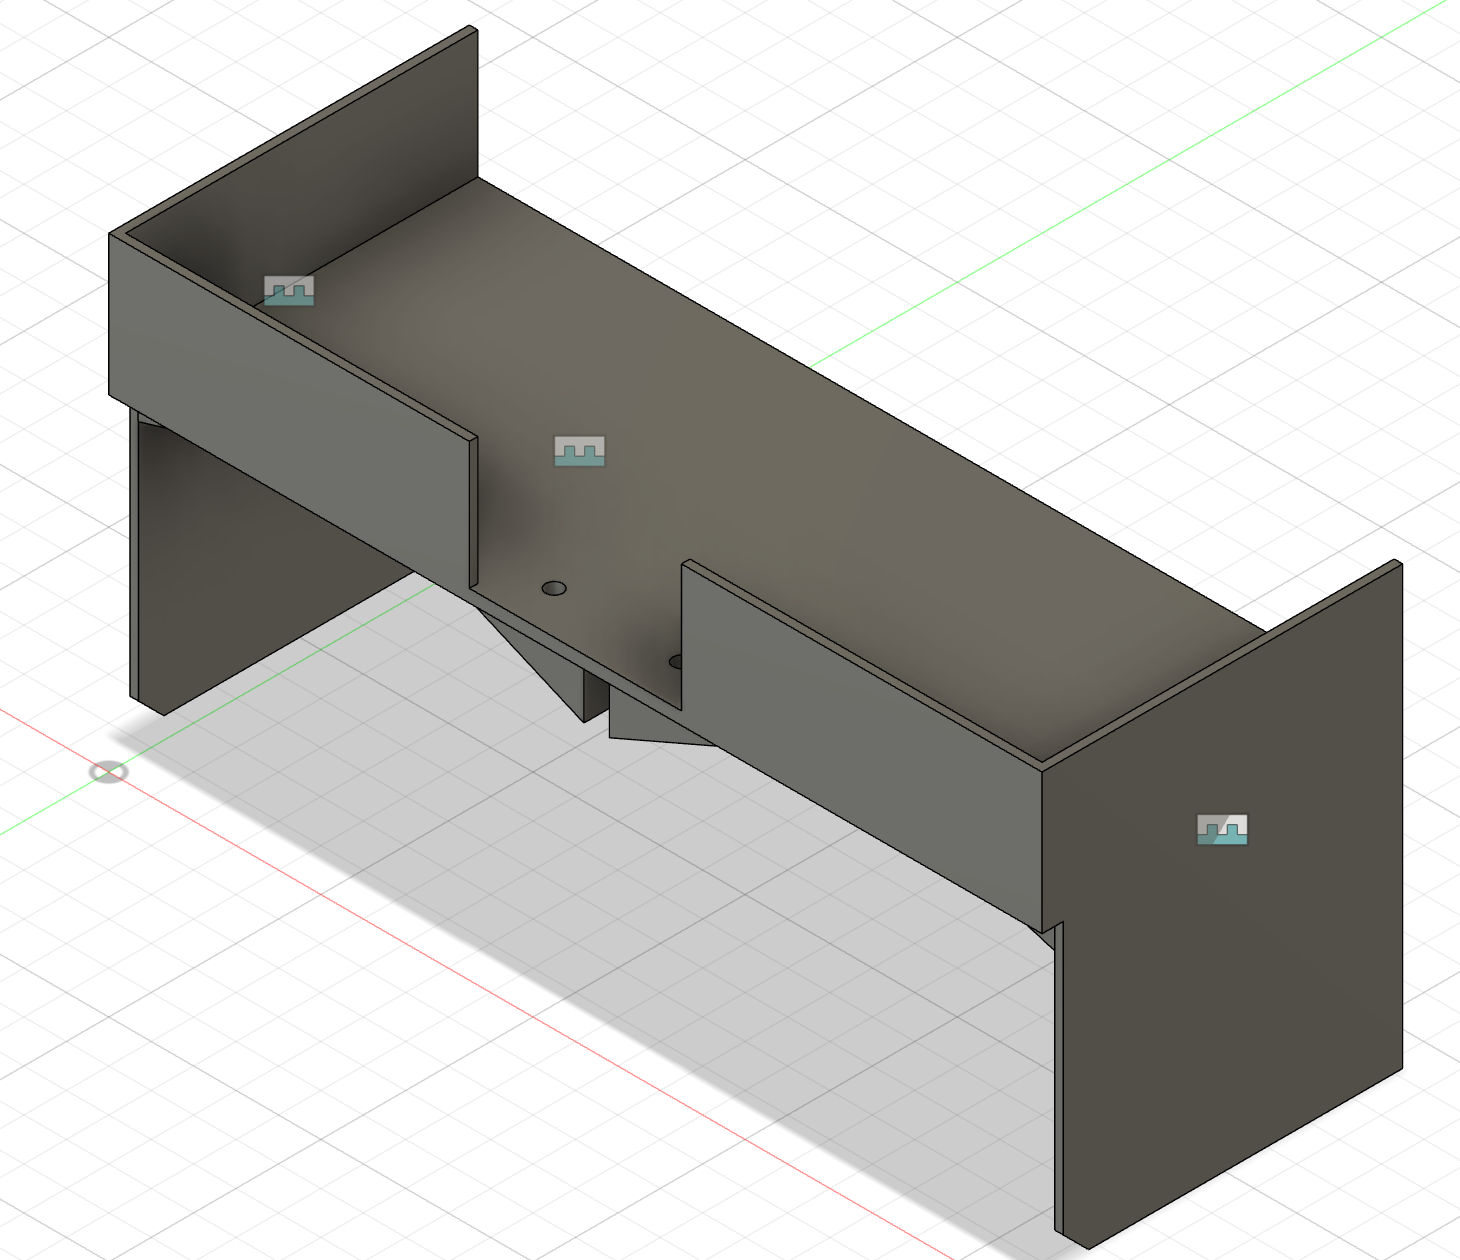
\includegraphics[width=1.0\textwidth]{./graf/upper.png}
    \caption{Zdjęcie przedstawiające stację dokującą oraz miejsce docelowe}
    \label{fig:stacja}
\end{figure}

\subsection{Warunki początkowe}

Ze względu na charakter pracy oraz sposób nawigacji oparty na uproszczonej odometrii przy użyciu enkoderów inkrementalnych, robot wykazuje dużą wrażliwość na warunki początkowe. Warunki te, definiujące początkowe położenie robota względem środowiska, mają kluczowe znaczenie dla dokładności jego działania. Nieprawidłowe ustawienie w pozycji bazowej może prowadzić do znaczących błędów w dalszej pracy, takich jak nieprecyzyjne podjechanie do stacji podajnikowej. Nawet niewielkie odchylenia, np. kilka stopni od linii zerowej, mogą skutkować krytycznymi problemami, takimi jak brak możliwości pobrania obiektu.

W celu minimalizacji tych błędów robot korzysta ze stacji dokujących przy punktach kontrolnych, które umożliwiają korekcję pozycji, jednak zakres ich działania jest ograniczony i nie rozwiązuje problemu dużych odchyleń. Rozwiązaniem tego problemu jest zastosowanie wyraźnego szablonu lub prowadnicy, który zapewni precyzyjne ustawienie robota w pozycji bazowej. Takie podejście znacząco zmniejsza ryzyko błędów wynikających z nieścisłości w ręcznym ustawianiu robota. % Podsumowanie i wnioski

\chapter{Spis skrótów i symboli}

\begin{itemize}
\item[CSI] szeregowy interfejs kamery (ang. \english{Camera Serial Interface})
\item[OpenCV] otwarta biblioteka wizji komputerowej(ang. \english{Open Source Computer Vision Library} )
\item[$N$] liczebność zbioru danych
\item[$\mu$] stopnień przyleżności do zbioru
\item[$\mathbb{E}$] zbiór krawędzi grafu
\item[$\mathcal{L}$] transformata Laplace'a 
\end{itemize}
 % Podsumowanie i wnioski
\backmatter

% \bibliographystyle{plplain}  %     bibtex
% \bibliography{biblio/biblio} % bibtex
\printbibliography           % biblatex
\addcontentsline{toc}{chapter}{Bibliografia}


\begin{appendices}

% TODO
\chapter{Spis skrótów i symboli}

\subsubsection*{Skróty ogólne}

\begin{itemize}
    \item[SBC] - Komputer jednopłytkowy (ang. \textit{Single Board Computer}), wykorzystywany jako główna jednostka obliczeniowa robota.
    \item[CSI] - Szeregowy interfejs kamery (ang. \textit{Camera Serial Interface}), umożliwiający połączenie kamery z komputerem SBC.
    \item[PID] - Regulator proporcjonalno-całkująco-różniczkujący (ang. \textit{Proportional-Integral-Derivative}), stosowany w systemach sterowania.
    \item[IDE] - Zintegrowane środowisko programistyczne (ang. \textit{Integrated Development Environment}), służące do programowania i debugowania kodu.
    \item[IMU] - Jednostka pomiaru inercyjnego (ang. \textit{Inertial Measurement Unit}), mierząca przyspieszenia liniowe i kątowe.
    \item[UML] - Diagram języka modelowania UML (ang. \textit{Unified Modeling Language}), wykorzystywany do wizualizacji systemów.
    \item[OpenCV] - Otwarte źródło biblioteki wizji komputerowej (ang. \textit{Open Source Computer Vision Library}), stosowanej do analizy obrazów.
    \item[git] - System kontroli wersji umożliwiający śledzenie zmian w kodzie oraz zarządzanie repozytoriami.
    \item[HDMI] - Interfejs multimedialny o wysokiej rozdzielczości (ang. \textit{High-Definition Multimedia Interface}), stosowany do przesyłania obrazu i dźwięku.
    \item[LED] -  dioda emitująca światło (ang. \english{Light-Emmiting Diode})
    \item[GPIO] - Ogólne wejścia/wyjścia cyfrowe (ang. \textit{General Purpose Input/Output}), używane do sterowania zewnętrznymi urządzeniami.
    \item[CSS] - Kaskadowe arkusze stylów (ang. \textit{Cascading Style Sheets}), używane do stylizacji stron internetowych.
    \item[PWM] - Modulacja szerokości impulsu (ang. \textit{Pulse Width Modulation}), wykorzystywana do sterowania silnikami i innymi urządzeniami.
    \item[USB] - Uniwersalna magistrala szeregowa (ang. \textit{Universal Serial Bus}), stosowana do podłączania urządzeń peryferyjnych.
    \item[SLAM] - Jednoczesna lokalizacja i mapowanie (ang. \textit{Simultaneous Localization and Mapping}), technologia używana w robotyce mobilnej.
    \item[LiDAR] - Detekcja i pomiar światła (ang. \textit{Light Detection and Ranging}), technologia służąca do tworzenia map 3D.
    \item[ROS2] - Robotyczny system operacyjny w wersji 2 (ang. \textit{Robot Operating System 2}), platforma do projektowania i sterowania robotami.
    \item[Docker] - Narzędzie do konteneryzacji, które umożliwia tworzenie, zarządzanie i uruchamianie aplikacji w izolowanych środowiskach. 
\end{itemize}

\subsubsection*{Symbole dotyczące regulatora PID}

\begin{itemize}
    \item[\(e_u\)] - Uchyb w stanie ustalonym, definiujący różnicę między wartością zadaną a rzeczywistą w stanie ustalonym.
    \item[\(e(t)\)] - Funkcja opisująca uchyb w czasie.
    \item[\(K_p\)] - Wzmocnienie członu proporcjonalnego.
    \item[\(K_i\)] - Wzmocnienie członu całkującego.
    \item[\(K_d\)] - Wzmocnienie członu różniczkującego.
    \item[\(E(s)\)] - Uchyb w dziedzinie operatorowej.
    \item[\(\mathcal{L}\)] - Operator Laplace’a, używany w analizie systemów dynamicznych.
    \item[\(y_{set}\)] - Wartość zadana (referencyjna).
    \item[\(y(t)\)] - Wyjście układu regulacji w funkcji czasu.
    \item[\(u(t)\)] - Funkcja sterująca regulatora PID w dziedzinie czasu.
    \item[\(U(s)\)] - Funkcja sterująca w dziedzinie operatorowej.
\end{itemize}

\subsubsection*{Symbole dotyczące odometrii oraz napędu różnicowego}

\begin{itemize}
    \item[\(\omega\)] - Prędkość kątowa platformy mobilnej.
    \item[\(\upsilon\)] - Prędkość liniowa platformy.
    \item[\(\upsilon_{r, l}\)] - Prędkości liniowe odpowiednio prawego i lewego koła.
    \item[\(b\)] - Odległość między osiami kół platformy.
    \item[\(x , y\)]  - Współrzędne środka masy platformy.
    \item[\(\theta\)]  - Orientacja platformy względem układu współrzędnych.
    \item[\(c_m\)] - Współczynnik przeliczania impulsów enkodera na odległość.
    \item[\(D_n\)] - Nominalna średnica kół.
    \item[\(C_e\)] - Rozdzielczość enkodera (impulsy na obrót).
    \item[\(n\)] - Przełożenie układu napędowego.
    \item[\(\Delta U_{R/L, I}\)] - Przebyta odległość przez prawe/lewe koło w czasie \(I\).
    \item[\(N_{R/L, I}\)] - Liczba impulsów zliczonych przez enkodery prawego/lewego koła w czasie \(I\).
\end{itemize}

\subsubsection*{Skróty oraz terminy dotyczące wizji komputerowej}

\begin{itemize}
    \item[Model RGB] - Model przestrzeni barw definiowany przez składowe: czerwony (\textit{Red}), zielony (\textit{Green}), niebieski (\textit{Blue}).
    \item[Model HSV] - Model przestrzeni barw definiowany przez odcień (\textit{Hue}), nasycenie (\textit{Saturation}), jasność (\textit{Value}).
    \item[Model YCrCb] - Model przestrzeni barw oddzielający luminancję (\textit{Y}) od chrominancji (\textit{Cr, Cb}).
    \item[K-means] - Algorytm grupowania danych, używany m.in. do segmentacji obrazów na podstawie kolorów.
    \item[Watershed] - Algorytm segmentacji obrazów oparty na analizie gradientów, wydzielający regiony o podobnych właściwościach.
\end{itemize}
 % Spis skrótów i symboli

% % TODO
% \chapter{Źródła}

Jeżeli w pracy konieczne jest umieszczenie długich fragmentów kodu źródłowego, należy je przenieść w to miejsce.

\begin{lstlisting}
if (_nClusters < 1)
	throw std::string ("unknown number of clusters");
if (_nIterations < 1 and _epsilon < 0)
	throw std::string ("You should set a maximal number of iteration or minimal difference -- epsilon.");
if (_nIterations > 0 and _epsilon > 0)
	throw std::string ("Both number of iterations and minimal epsilon set -- you should set either number of iterations or minimal epsilon.");
\end{lstlisting}


% % % % % % % % % % % % % % % % % % % % % % % % % % % % % % % % % % % 
% Pakiet minted wymaga odkomentowania w pliku config/settings.tex   %
% importu pakietu minted: \usepackage{minted}                       %
% i specjalnego kompilowania:                                       %
% pdflatex -shell-escape praca                                      %
% % % % % % % % % % % % % % % % % % % % % % % % % % % % % % % % % % % 

%\begin{minted}[linenos,breaklines,frame=lines]{c++}
%if (_nClusters < 1)
%   throw std::string ("unknown number of clusters");
%if (_nIterations < 1 and _epsilon < 0)
%   throw std::string ("You should set a maximal number of iteration or minimal difference -- epsilon.");
%if (_nIterations > 0 and _epsilon > 0)
%   throw std::string ("Both number of iterations and minimal epsilon set -- you should set either number of iterations or minimal epsilon.");
%\end{minted}
 % Źródła

% TODO
\chapter{Lista dodatkowych plików, uzupełniających tekst pracy} 


W systemie do pracy dołączono dodatkowe pliki zawierające:
\begin{itemize}
\item film pokazujący działanie opracowanego oprogramowania lub zaprojektowanego i~wykonanego urządzenia,
\end{itemize}
 % Lista dodatkowych plików, uzupełniających tekst pracy

% \listoftables
% \addcontentsline{toc}{chapter}{Spis tabel}

\end{appendices}

\end{document}


%% Finis coronat opus.